\chapter{Realisierung eines Prototyps}

Für das Projekt \doublequotes{UrbanLife+} soll nun ein Prototyp einer mobilen Anwendung realisiert werden. An der Universität Leipzig wird bereits eine mobile Anwendung mit Google's Development Kit \emph{Flutter} entwickelt. Dieses dient dazu, plattformübergreifende Anwendungen für beispielsweise iOS und Android zu programmieren. Um eine App für die Apple Watch zu programmieren, existieren jedoch keine Tools. Soll eine Anwendung auf der Apple Watch laufen, muss auf Apple's eigene Programmiersprache \emph{Swift} zurückgegriffen werden.

Wir wollen ein \doublequotes{Human-centred Design} für unsere App erreichen und folgen somit der Norm ISO 9241-210 (vgl. \autoref{dia:human-centered-design-process}). Der Code der App lässt sich unter \url{https://github.com/hhontheim/UrbanLifePlusApp} herunterladen.

\section{Beschreiben des Nutzungskontexts}

Um den Nutzungskontext zu verstehen, verschaffen wir uns zunächst einen Überblick über das Projekt.

Das Ziel des Projekts ist es, die Teilhabe von Senioren im öffentlichen Raum zu verbessern. Dies wird dadurch versucht zu erreicht, indem städtebauliche Objekte in \acp{SSO} verwandelt werden. Diese sollen die Senioren bedarfsgerecht unterstützen und es ihnen ermöglichen, sich sicher in der Stadt zu bewegen. Durch die Bereitstellung von \emph{Informationsstrahlern} soll das Gewahrsein der Nutzer erhöht werden. Um einem Nutzer die Möglichkeit zu geben, sich an diesen Informationsstrahlern anzumelden, braucht es ein Lösung \cite{Fietkau:2020:FuE-Vorhaben-Informationsstrahler---Backend,Fietkau:2020:FuE-Vorhaben-Informationsstrahler---MTI-Gestaltung}.

\section{Spezifizierung der Anforderungen}

Zur Identifikation sind mehrere Möglichkeiten denkbar. Zum einen kann der Nutzer ein Gerät bei sich tragen, das konstant eine Bluetooth-UUID sendet. Dies kann zum Beispiel ein \emph{iBeacon} oder Smartphone sein. Da ein \emph{iBeacon} jedoch keine Informationen empfangen kann, benötigt das \ac{SSO} dazu eine Verbindung zum Internet, um die Daten des Nutzers abzurufen. Möchte man eine Lösung, die ohne Internetverbindung funktioniert, müssen Daten bidirektional zwischen dem \ac{SSO} und dem Nutzer übertragen werden können. Somit kommt die \emph{iBeacon}-Technologie nicht infrage.

Wir wollen, dass unsere Anwendung auf der Apple Watch laufen kann. Der Nutzer soll sein Profil auf einem iPhone mit gekoppelter Apple Watch verwalten und mit \ac{SSO} in der Nähe kommunizieren können. In \autoref{sec:bluetooth} haben wir bereits die verschiedenen Arten der Kommunikation über Bluetooth kennengelernt. Da wir uns mit dem \ac{SSO} sowohl über das iPhone, als auch die Apple Watch, verbinden wollen, muss das \ac{SSO} also als Bluetooth \emph{Peripheral} agieren. Dadurch können wir uns mit unseren mobilen Geräten am \ac{SSO} anmelden und mit diesem Daten austauschen.

Innerhalb der beiden Apps soll der Nutzer sein Profil verwalten können. Die Daten über das \emph{WatchConnectivity}-Framework zwischen den Geräten synchron gehalten und über das iPhone im \emph{Key-Value}-Speicher der iCloud als Backup abgelegt werden.

Die iPhone-App soll zudem die Möglichkeit besitzen, Push-Benachrichtigungen zu empfangen und einen Support-Chat beinhalten.

\section{Entwickeln einer Gestaltungslösung}

Bei der Implementierung der App halten wir uns an die Richtlinien und Best Practices aus \autoref{sec:guidelines}. Apple stellt für die Entwicklung von Apps eigene Richtlinien zur Verfügung, die \citetitle{Apple::Human-Interface-Guidelines} \cite{Apple::Human-Interface-Guidelines}. Diese geben Entwicklern spezielle Richtlinien vor, die Apple eingehalten haben möchte. Bei Veröffentlichung im App Store müssen diese Richtlinien zwingend eingehalten werden.

\subsection{User Interface des iPhone}

Öffnet der Nutzer die Anwendung zum ersten Mal, sieht er einen Begrüßungs-Bildschirm (\autoref{fig:app:ios:loginNoAccount}) und wird dazu aufgefordert, sich einen Account zu erstellen. Wir nutzen hier die mit iOS 13 eingeführte \emph{Single-Sign-On}-Lösung \doublequotes{Sign in with Apple}. Um die Nutzer nicht zu überfordern, verzichten wir auf die \doublequotes{klassische} Passwort-Variante. Apple nutzt hierfür die Daten der Apple-ID und stellt uns eine Nutzer-ID, einen Token und einen Code bereit, mit dem wir die Authentisierung des Nutzers gegenüber Apple überprüfen können. Dieses ähnelt dem \emph{OAuth}-Protokoll. Für den Nutzer hat es den Vorteil, dass er zusätzlich zu \emph{keinem Passwort}, das er sich merken muss, seine private Mailadresse verstecken kann. Apple betreibt hierfür einen \emph{Relay}-Service, der Mails an die privaten Adressen der Nutzer weiterleiten kann. Hat der Nutzer bereits einen Account erstellt, sieht der Login-Screen wie in \autoref{fig:app:ios:loginWithAccount} aus.

Ist der Nutzer angemeldet, zeigt \autoref{fig:app:ios:home}, wie die Startseite der App aussieht. Diese stellt zwei Schalter zur Verfügung, die für den automatischen Verbindungsaufbau der Geräte mit \ac{SSO} dienen und zwischen dem iPhone und der Apple Watch synchronisiert werden. Ist das iPhone mit einem \ac{SSO} verbunden, zeigt \autoref{fig:app:ios:homeConnected}, wie verbundene \ac{SSO} dargestellt werden. In diesem Fall wird ein \doublequotes{ULP Demo Device} angezeigt, das in \autoref{sec:esp32}  vorgestellt wird.

Über eine \emph{TabView} kann sich der Nutzer durch die App bewegen. Tippt er auf das Herz-Icon kommt er zu den persönlichen Präferenzen (\autoref{fig:app:ios:prefs}). Hier kann er festlegen, wie sich die \ac{SSO} bei einer Verbindung verhalten sollen. Unser \doublequotes{ULP Demo Device} hat die Möglichkeit, eine LED aufleuchten zu lassen. Die anderen Einstellungen dienen nur der Demonstration und haben keine Funktionalität.

In den Einstellungen (\autoref{fig:app:ios:settings}) hat der Nutzer mehrere Möglichkeiten. Entweder kann er die persönlichen Daten, wie in \autoref{fig:app:ios:profile} gezeigt, bearbeiten oder das Entwickler-Menü (\autoref{fig:app:ios:dev}) aufrufen. Dieses zeigt neben den Daten, die beim Authen\-tisierungs-Prozess von Apple bereitgestellt werden, auch die verbundenen Geräte an. Für den Fall, dass der Nutzer sich nicht automatisch mit den Geräten verbinden möchte (wie in \autoref{fig:app:ios:home}), werden alle Geräte in der Nähe angezeigt. Falls das iPhone jedoch den Sendebereich eines \emph{Peripherals} verlässt, verschwindet dieses nicht automatisch aus der Liste. iOS bietet hierfür keine direkte Unterstützung an.

Benötigt ein Nutzer Hilfe (\autoref{fig:app:ios:helpSheet}), hat er zwei Möglichkeiten. Zum einen nutzt die App das 3rd-Party-Framework \doublequotes{Customerly}\footnote{\url{https://www.customerly.io/}}. Dieses Framework stellt dem Nutzer eine Chat-Kommunikation zur Verfügung, die er benutzen kann, um direkte Hilfe zu erhalten.

Ein weiteres verwendetes 3rd-Party-Framework ist \doublequotes{Instabug}\footnote{\url{https://instabug.com/}}, welches in der kostenpflichtigen Version ebenfalls einen Chat bereitstellen würde. Da \doublequotes{Customerly} dies allerdings kostenfrei ermöglicht, wird \doublequotes{Instabug} hierfür nicht genutzt. Stattdessen dient es uns dazu, automatisch Fehlerdaten bei App-Abstürzen zu sammeln. \doublequotes{Instabug} kann ein Nutzer aber auch aktiv nutzen, über das er technische Probleme, wie \emph{Bugs} oder Verbesserungsvorschläge einreichen kann. Beide Frameworks erfüllen somit die \doublequotes{SMASH 11}-Anforderung aus \autoref{tab:smash-list}.

Da alle Daten des Nutzers auf dem iPhone gespeichert werden, soll es selbstverständlich auch die Möglichkeit geben, alle Daten zu löschen (\autoref{fig:app:ios:nukeSheet}). Will ein Nutzer alle Daten löschen, werden diese ebenfalls von der Apple Watch und der iCloud entfernt. Nach dem Löschvorgang wird \autoref{fig:app:ios:nuked} angezeigt, die Instruktionen zum Reset der App bereitstellt. Über \emph{Sign in with Apple} erhalten wir von Apple nur ein einziges Mal die Mailadresse! Wurde diese gelöscht, muss die Verknüpfung zwischen App und Apple-ID aufgehoben werden.

\subsection{User Interface der Apple Watch}

Da das Display der Apple Watch deutlich kleiner ist, wird auf die Texteingabe verzichtet. Die Apple Watch bekommt alle Daten vom iPhone. Erst wenn sich der Nutzer auf dem iPhone angemeldet hat, verschwindet der Login-Screen (\autoref{fig:app:watchos:loginNoAccount}, beziehungsweise \ref{fig:app:watchos:loginWithAccount}). Abbildungen \ref{fig:app:watchos:home1} bis \ref{fig:app:watchos:connectedTo} zeigen, wie die Schnittstelle des iPhone auf der Apple Watch aussieht. Von der Funktionalität unterscheidet sich die Apple Watch darin nicht.

\section{Evaluation der Gestaltungslösung}

Insgesamt wurde versucht, eine einfache und intuitive Benutzerschnittstelle zu realisieren. Orientiert hat sich der gesamte Entwicklungsprozess an den Erkenntnissen aus \autoref{sec:guidelines}. Mithilfe eines abschließenden Tests durch Nutzer der Zielgruppe, kann nun festgestellt werden, ob durch die Umsetzung die Gestaltungsanforderungen erfüllt wurden, oder eine weitere Iteration des Prozesses notwendig ist.

\section{Deployment der Anwendung}

Um die Anwendung auf einem physischen Geräten zu testen, wurde eine kleine \emph{Continuous Integration}-Pipeline aufgesetzt. Bei jedem \emph{Push} in das GitHub-Repository\footnote{\url{https://github.com/hhontheim/UrbanLifePlusApp}}, wird die aktuellste Version gebaut und zur Ad-Hoc-Installation auf \url{http://ulp.hontheim.net/} hochgeladen. Da Apple den App Store bekanntlicherweise nicht umgangen haben möchte, muss jedes iPhone und jede Apple Watch explizit für die App freigeschaltet werden. Wenn Sie die App testen möchten, öffnen Sie bitte einen \emph{Pull Request} für das Repository, und schreiben Sie die UUID/UDID der betroffenen Geräte in die \texttt{devices.txt}-Datei im Root-Verzeichnis. Alternativ können Sie mir die IDs auch per Mail zukommen lassen oder das Xcode-Projekt selber bauen.

\section{Prototyp eines SSO}\label{sec:esp32}

Zu Demonstrationszwecken wurde ein Breadbord mit drei ESP32-Modulen bestückt (\autoref{fig:esp:off}). Diese Chips der Marke \emph{Espressif Systems} besitzen eine eingebaute Bluetooth-Antenne. Im Code-Repository befindet sich der \texttt{C++}-Code, der mit der \emph{Arduino IDE} auf die Module geladen wurde. Jeder einzelne Chip sendet den \doublequotes{ULP Demo Service}\footnote{DIe UUID dieses Services lautet \texttt{F278E33F-D8F1-4F4B-8E04-885A5968FA11}.} aus und verfügt über eine LED. Die oberen beiden Module werden über eine externe Stromzufuhr versorgt, das untere über USB. Das untere Modul verfügt zudem über ein Display.

Wenn ein Modul angeschaltet wird, sendet es den Service und akzeptiert Verbindungen (\autoref{fig:esp:on}). Wenn der Nutzer auf dem iPhone oder der Apple Watch eine Verbindung herstellt, werden automatisch der Name und die ID des Nutzers (sichtbar in \autoref{fig:app:ios:dev}) übermittelt und im Display in \autoref{fig:esp:connected} angezeigt. Aktiviert der Nutzer die LED-Präferenz in der App, schalten sich die LEDs ein (\autoref{fig:esp:led}).

\begin{figure}[H]
	\centering
	\includegraphics[width=.8\textwidth]{./images/prototype/esp/off.png}
	\caption{\label{fig:esp:off}Der ausgeschaltete Prototyp mit drei Peripheriegeräten, einem Display und externer Stromversorgung.}
\end{figure}

\begin{figure}[H]
	\centering
	\includegraphics[width=.8\textwidth]{./images/prototype/esp/on.png}
	\caption{\label{fig:esp:on}Der eingeschaltete Prototyp. Die Geräte akzeptieren Verbindungen.}
\end{figure}

\begin{figure}[H]
	\centering
	\includegraphics[width=.8\textwidth]{./images/prototype/esp/connected.png}
	\caption{\label{fig:esp:connected}Nutzer hat Verbindung hergestellt. Übermittelte Daten werden im Display angezeigt.}
\end{figure}

\begin{figure}[H]
	\centering
	\includegraphics[width=.8\textwidth]{./images/prototype/esp/led.png}
	\caption{\label{fig:esp:led}Nutzer ist verbunden und hat die LED-Präferenz in der App aktiviert.}
\end{figure}
\clearpage

\section{Screenshots der Anwendungen}

In diesem Kapitel werden die Screenshots der beiden Apps gezeigt.

\subsection{iOS App}

\begin{minipage}{.45\textwidth}
	\begin{figure}[H]
		\centering
		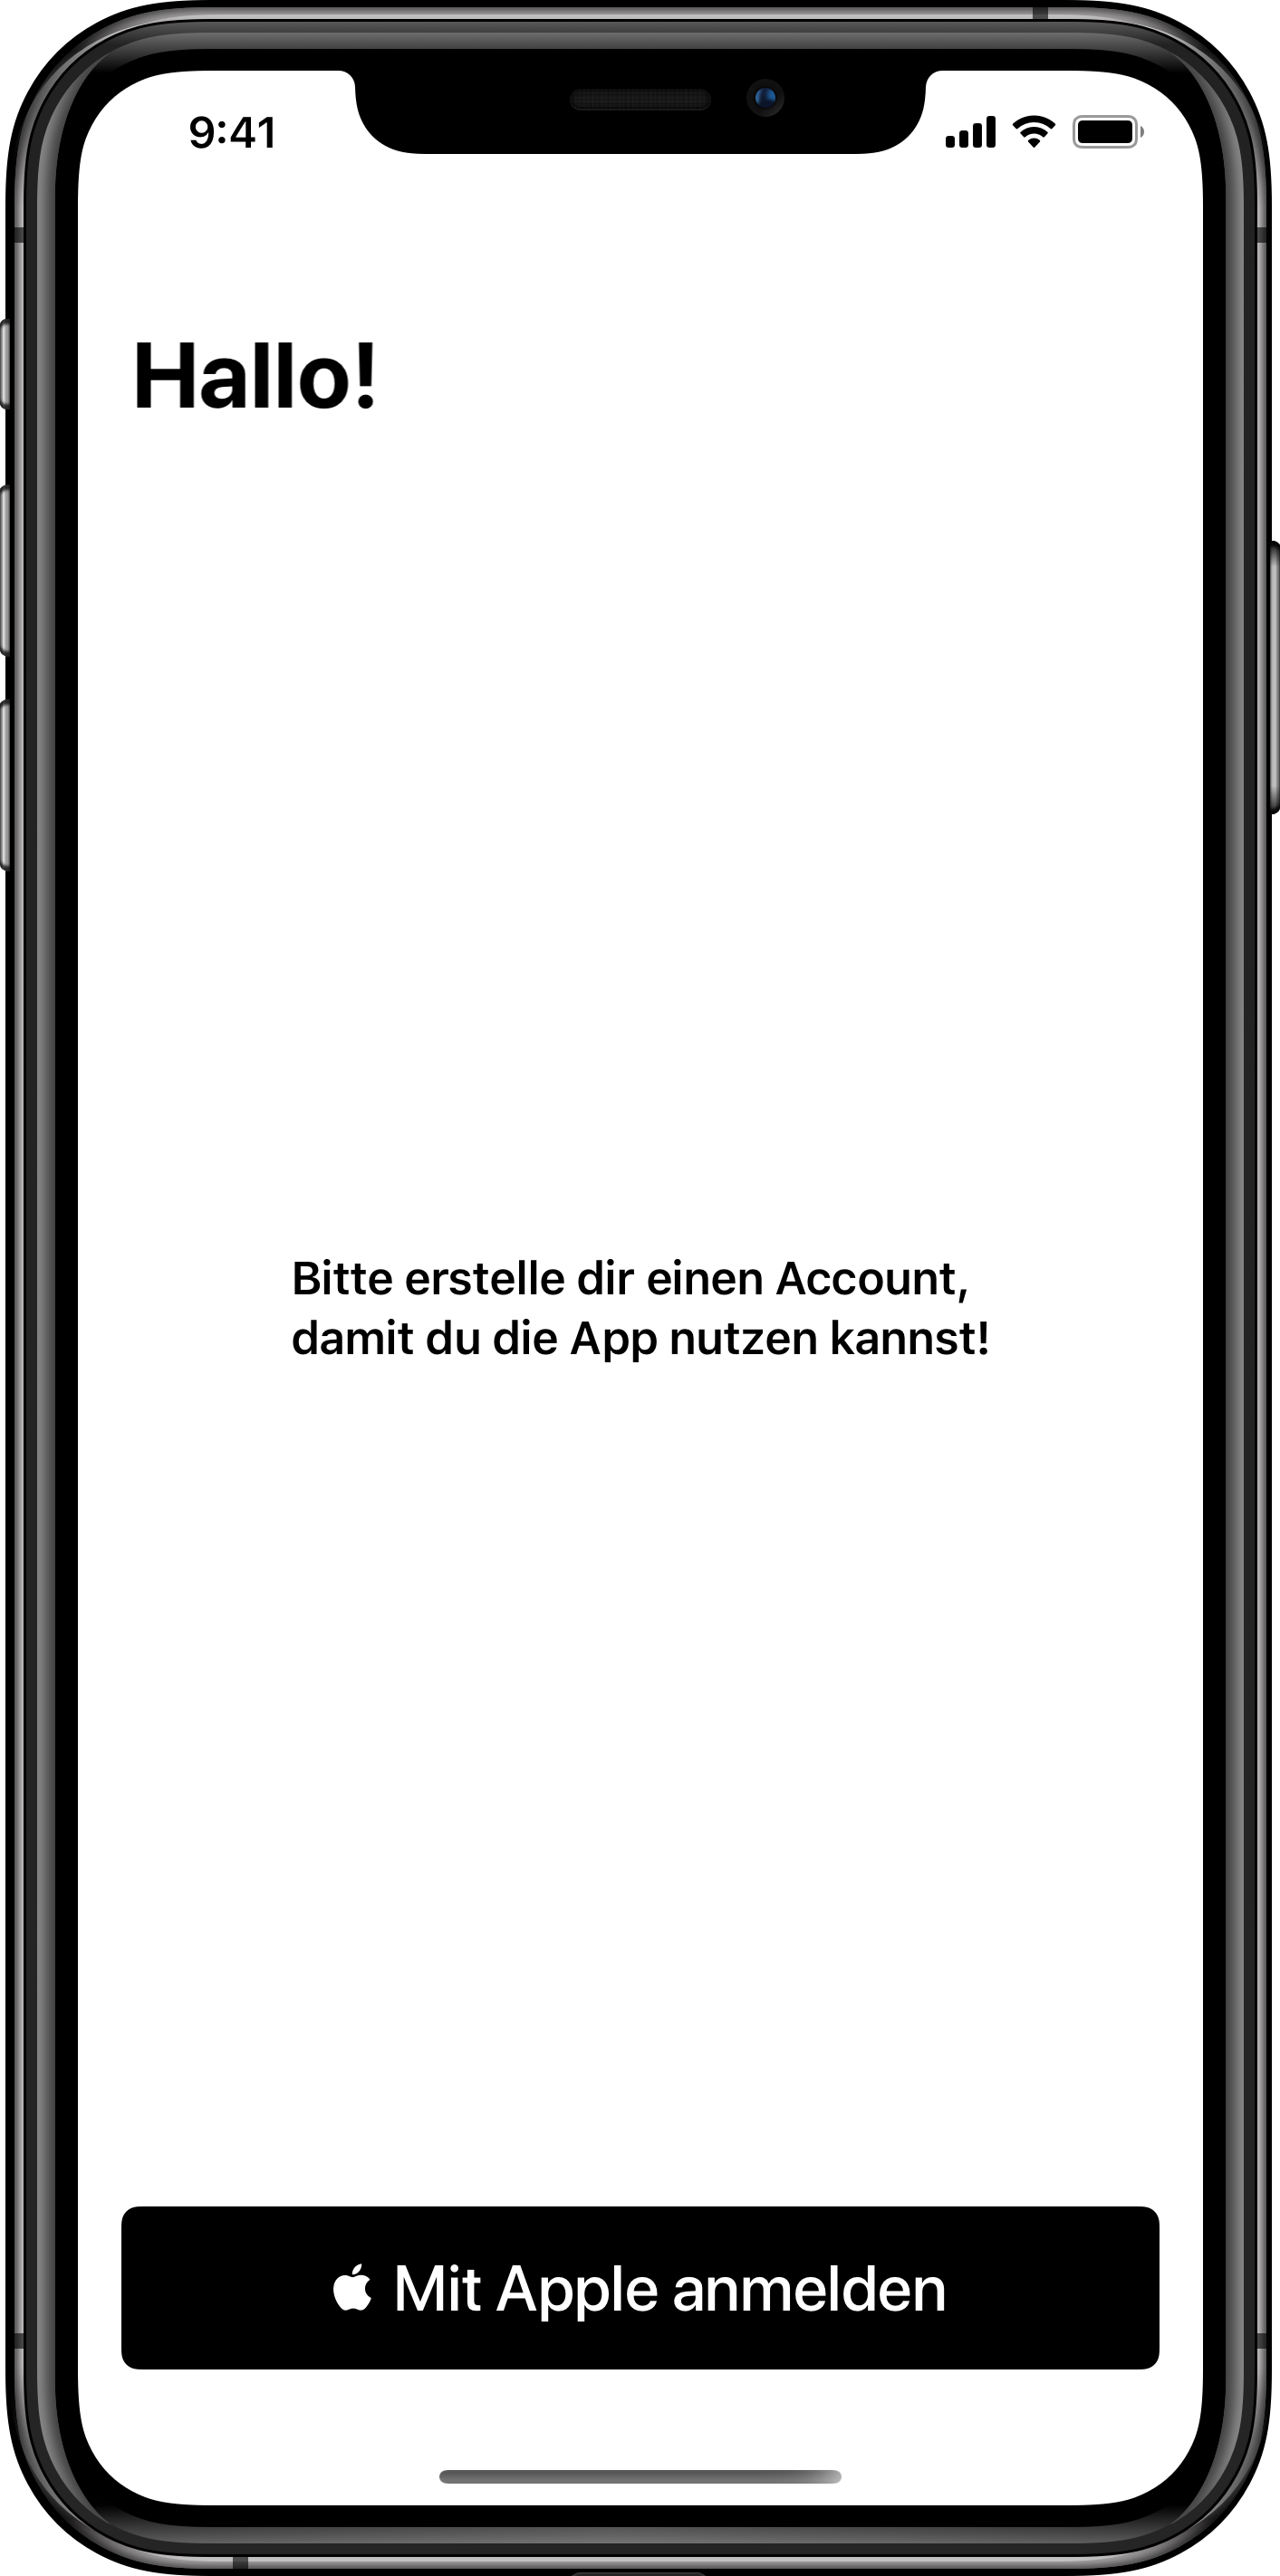
\includegraphics[width=.68\textwidth]{./images/prototype/ios/loginNoAccount.png}
		\caption{\label{fig:app:ios:loginNoAccount}Login-Screen. Benutzer hat noch keinen Account angelegt.}
	\end{figure}
\end{minipage}\hfill
\begin{minipage}{.45\textwidth}
	\begin{figure}[H]
		\centering
		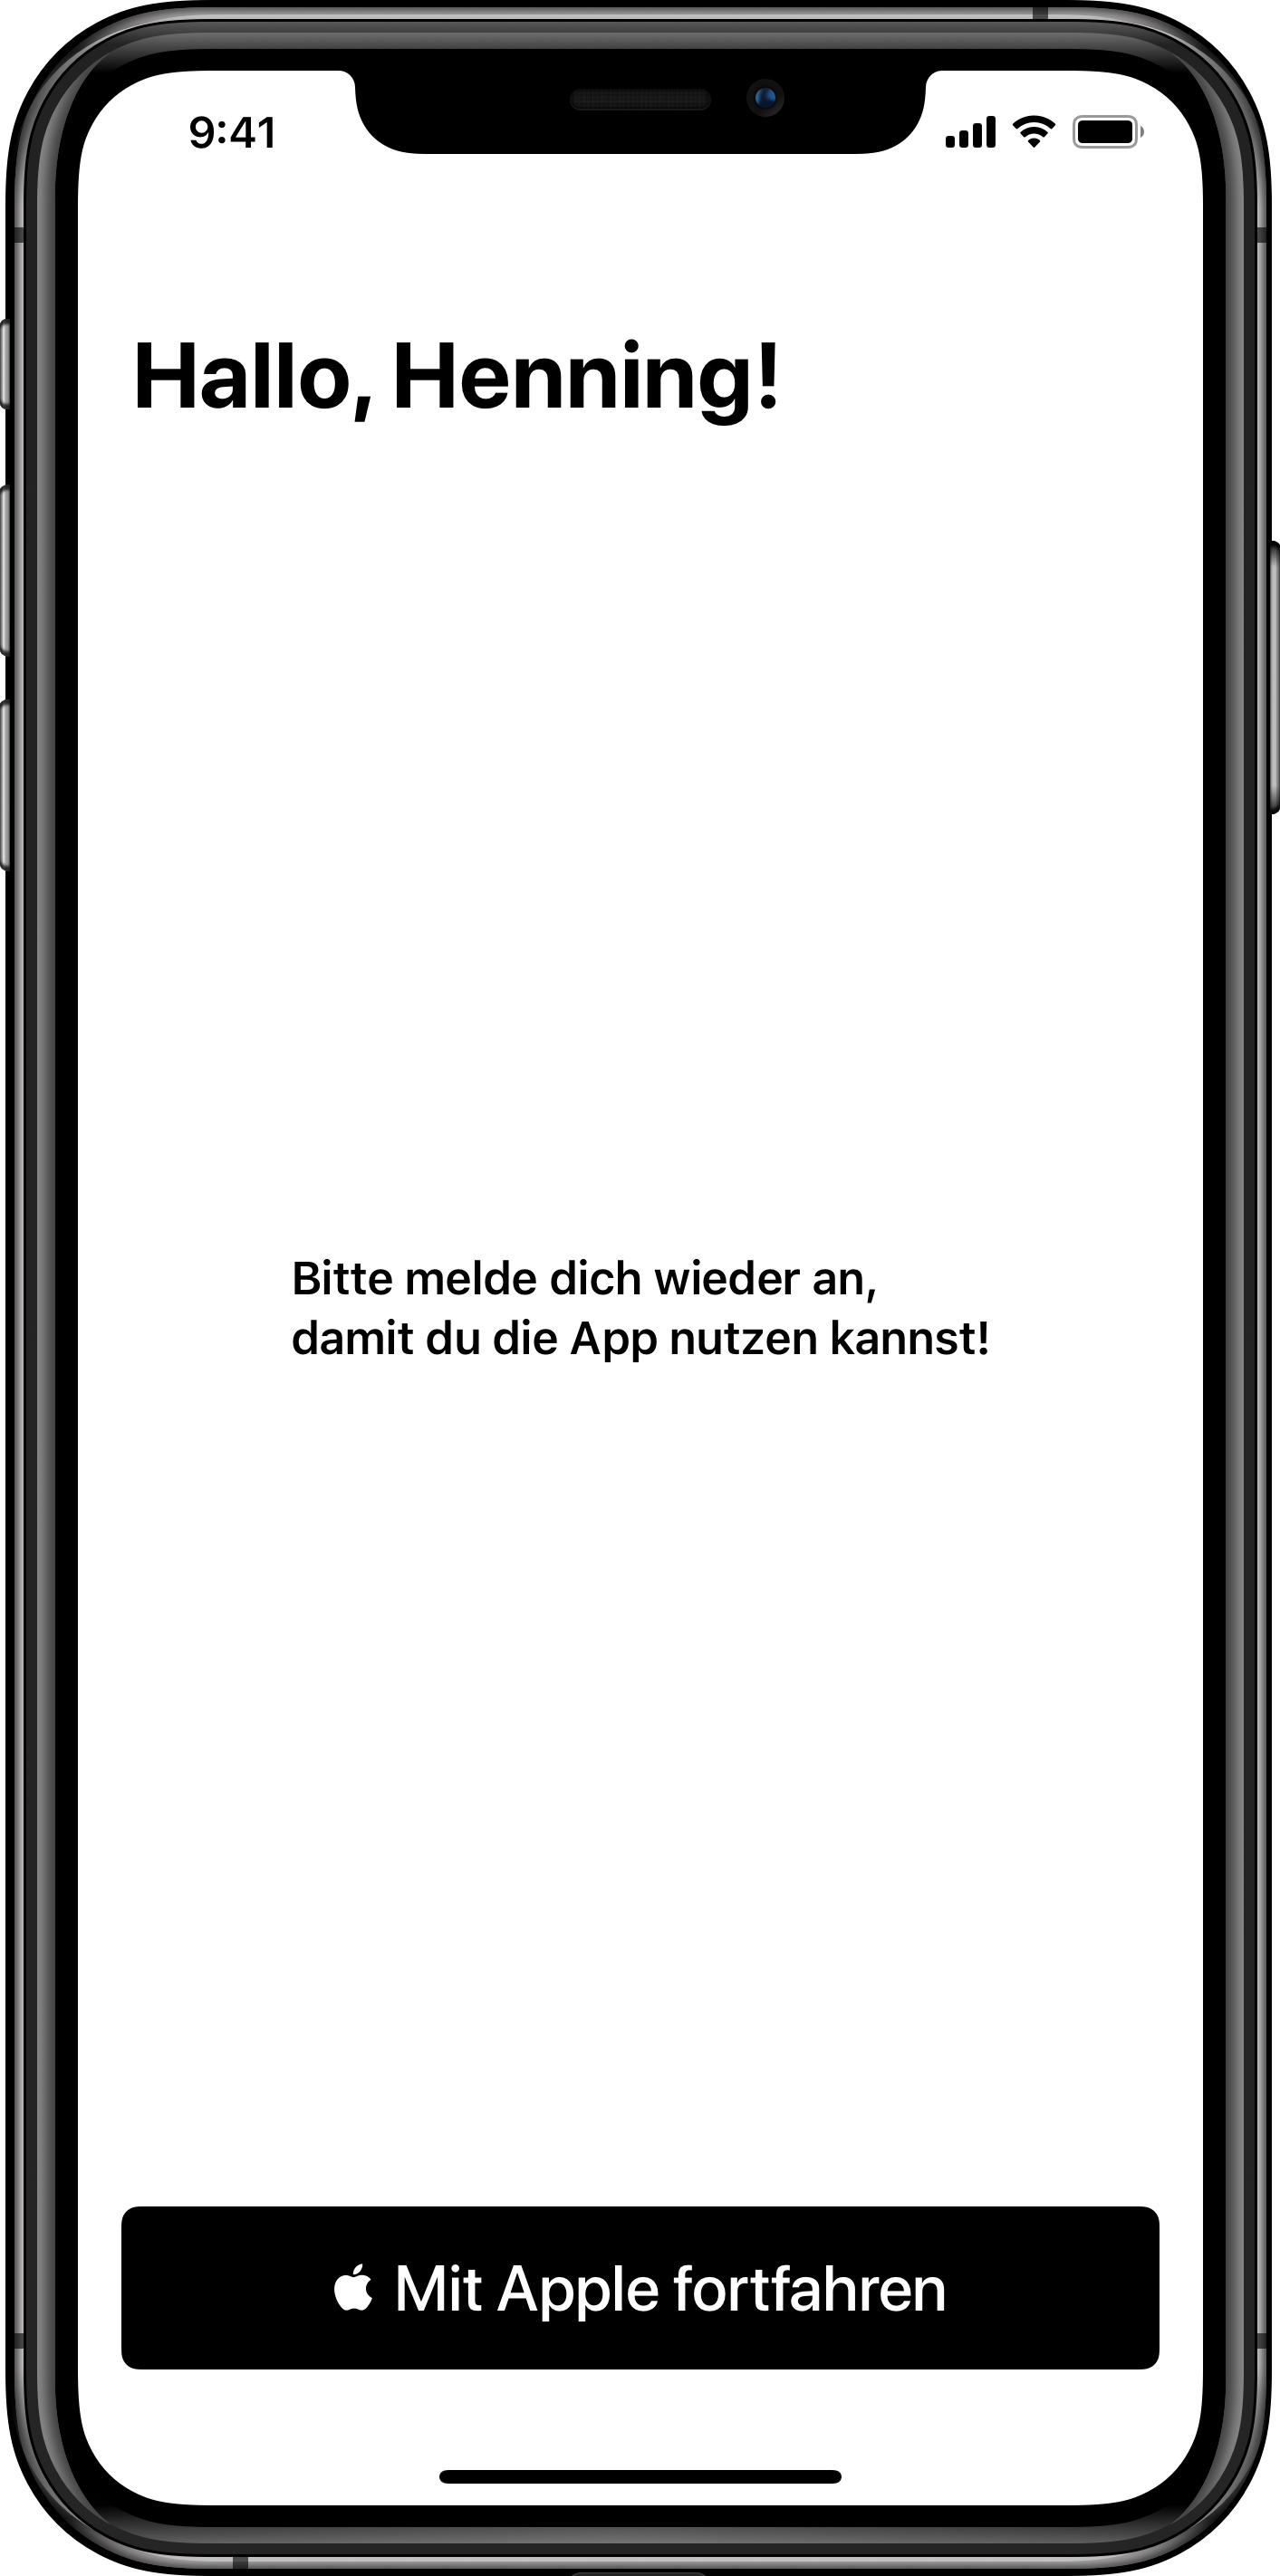
\includegraphics[width=.68\textwidth]{./images/prototype/ios/loginWithAccount.png}
		\caption{\label{fig:app:ios:loginWithAccount}Login-Screen. Benutzer hat bereits einen Account angelegt.}
	\end{figure}
\end{minipage}\clearpage

\begin{minipage}{.45\textwidth}
	\begin{figure}[H]
		\centering
		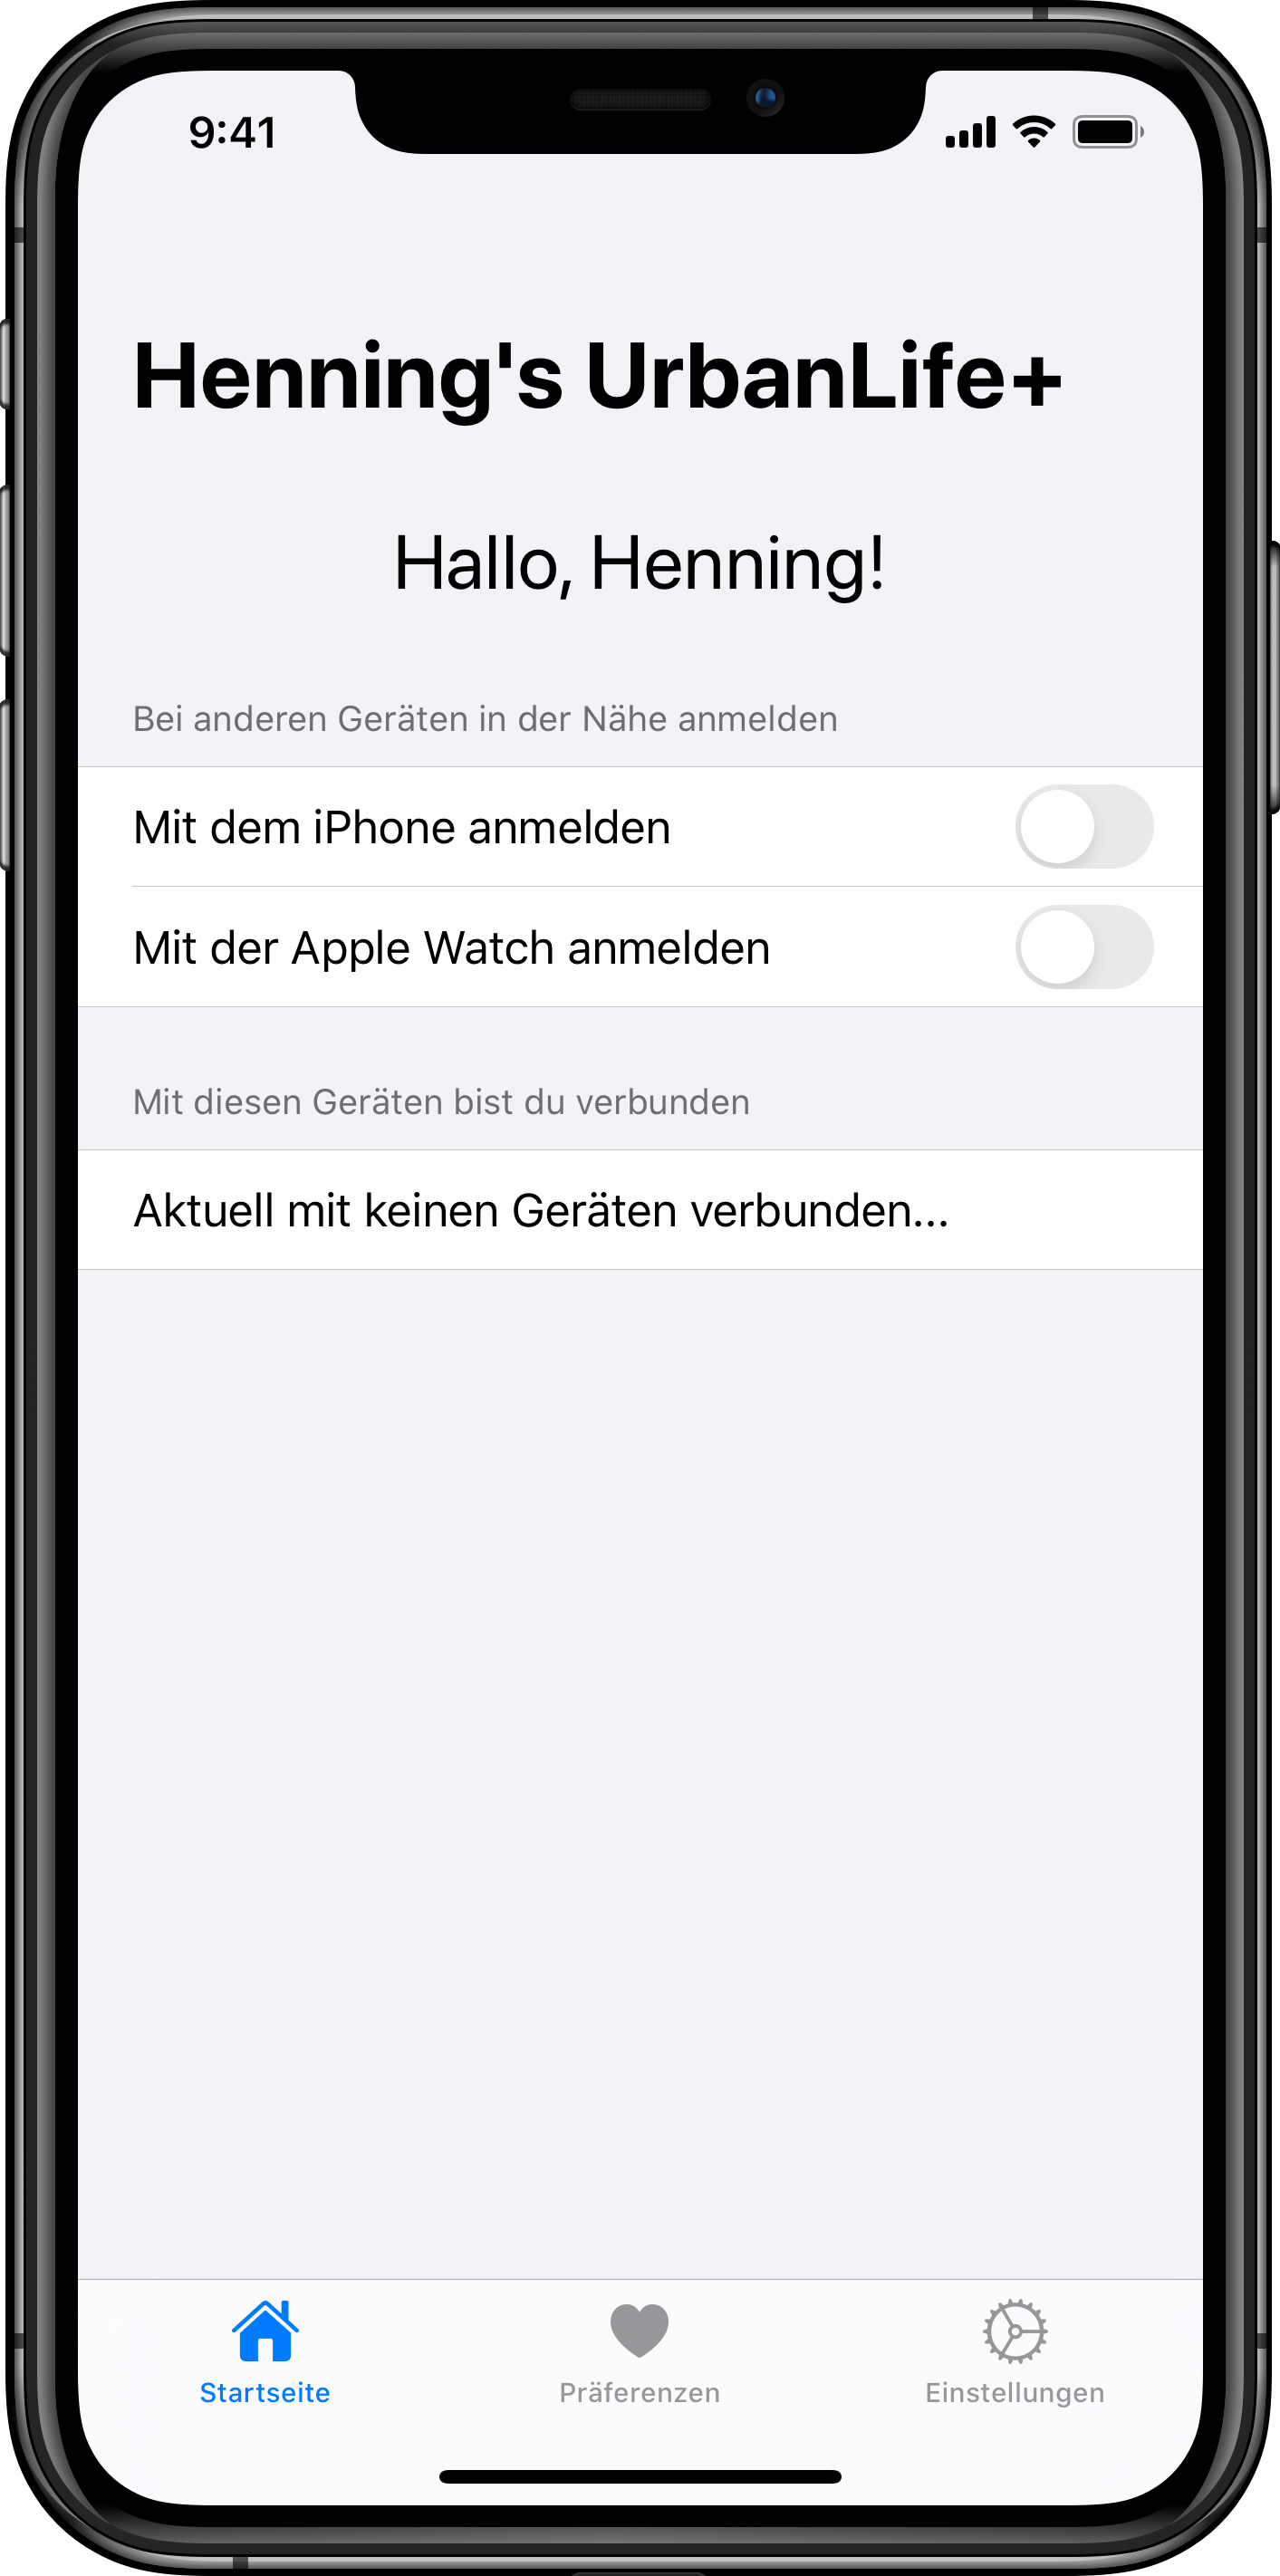
\includegraphics[width=.68\textwidth]{./images/prototype/ios/home.png}
		\caption{\label{fig:app:ios:home}Startseite. Kein Gerät verbunden.}
	\end{figure}
\end{minipage}\hfill
\begin{minipage}{.45\textwidth}
	\begin{figure}[H]
		\centering
		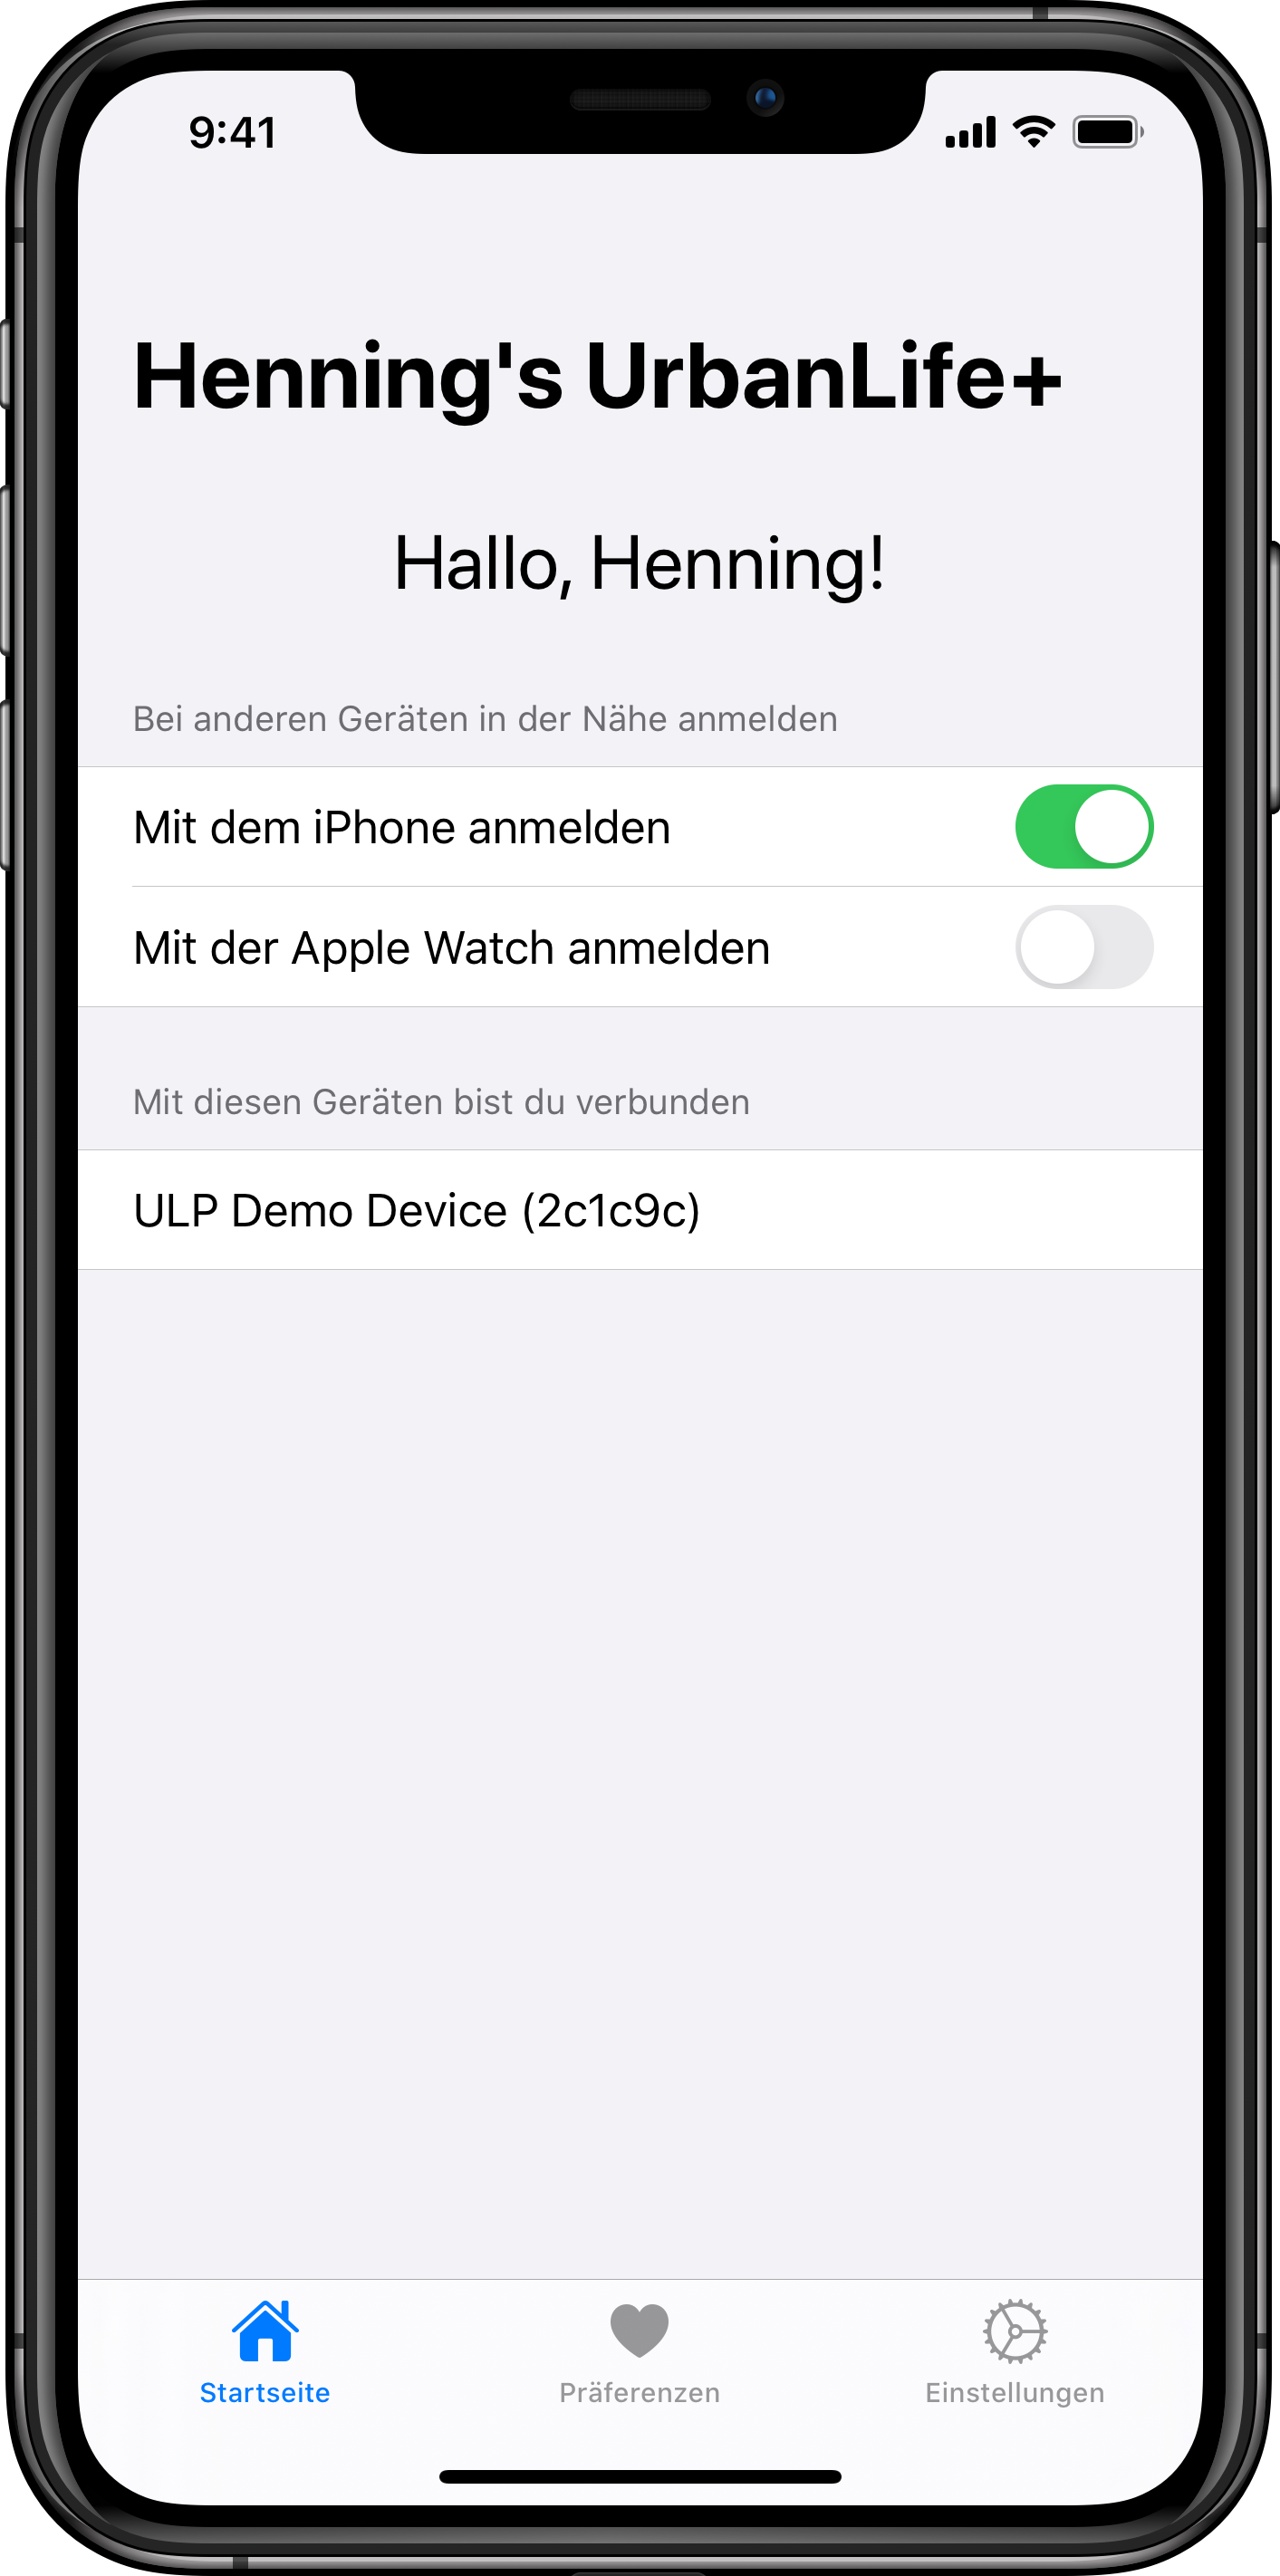
\includegraphics[width=.68\textwidth]{./images/prototype/ios/homeConnected.png}
		\caption{\label{fig:app:ios:homeConnected}Startseite mit verbundenem Gerät.}
	\end{figure}
\end{minipage}

\begin{minipage}{.45\textwidth}
	\begin{figure}[H]
		\centering
		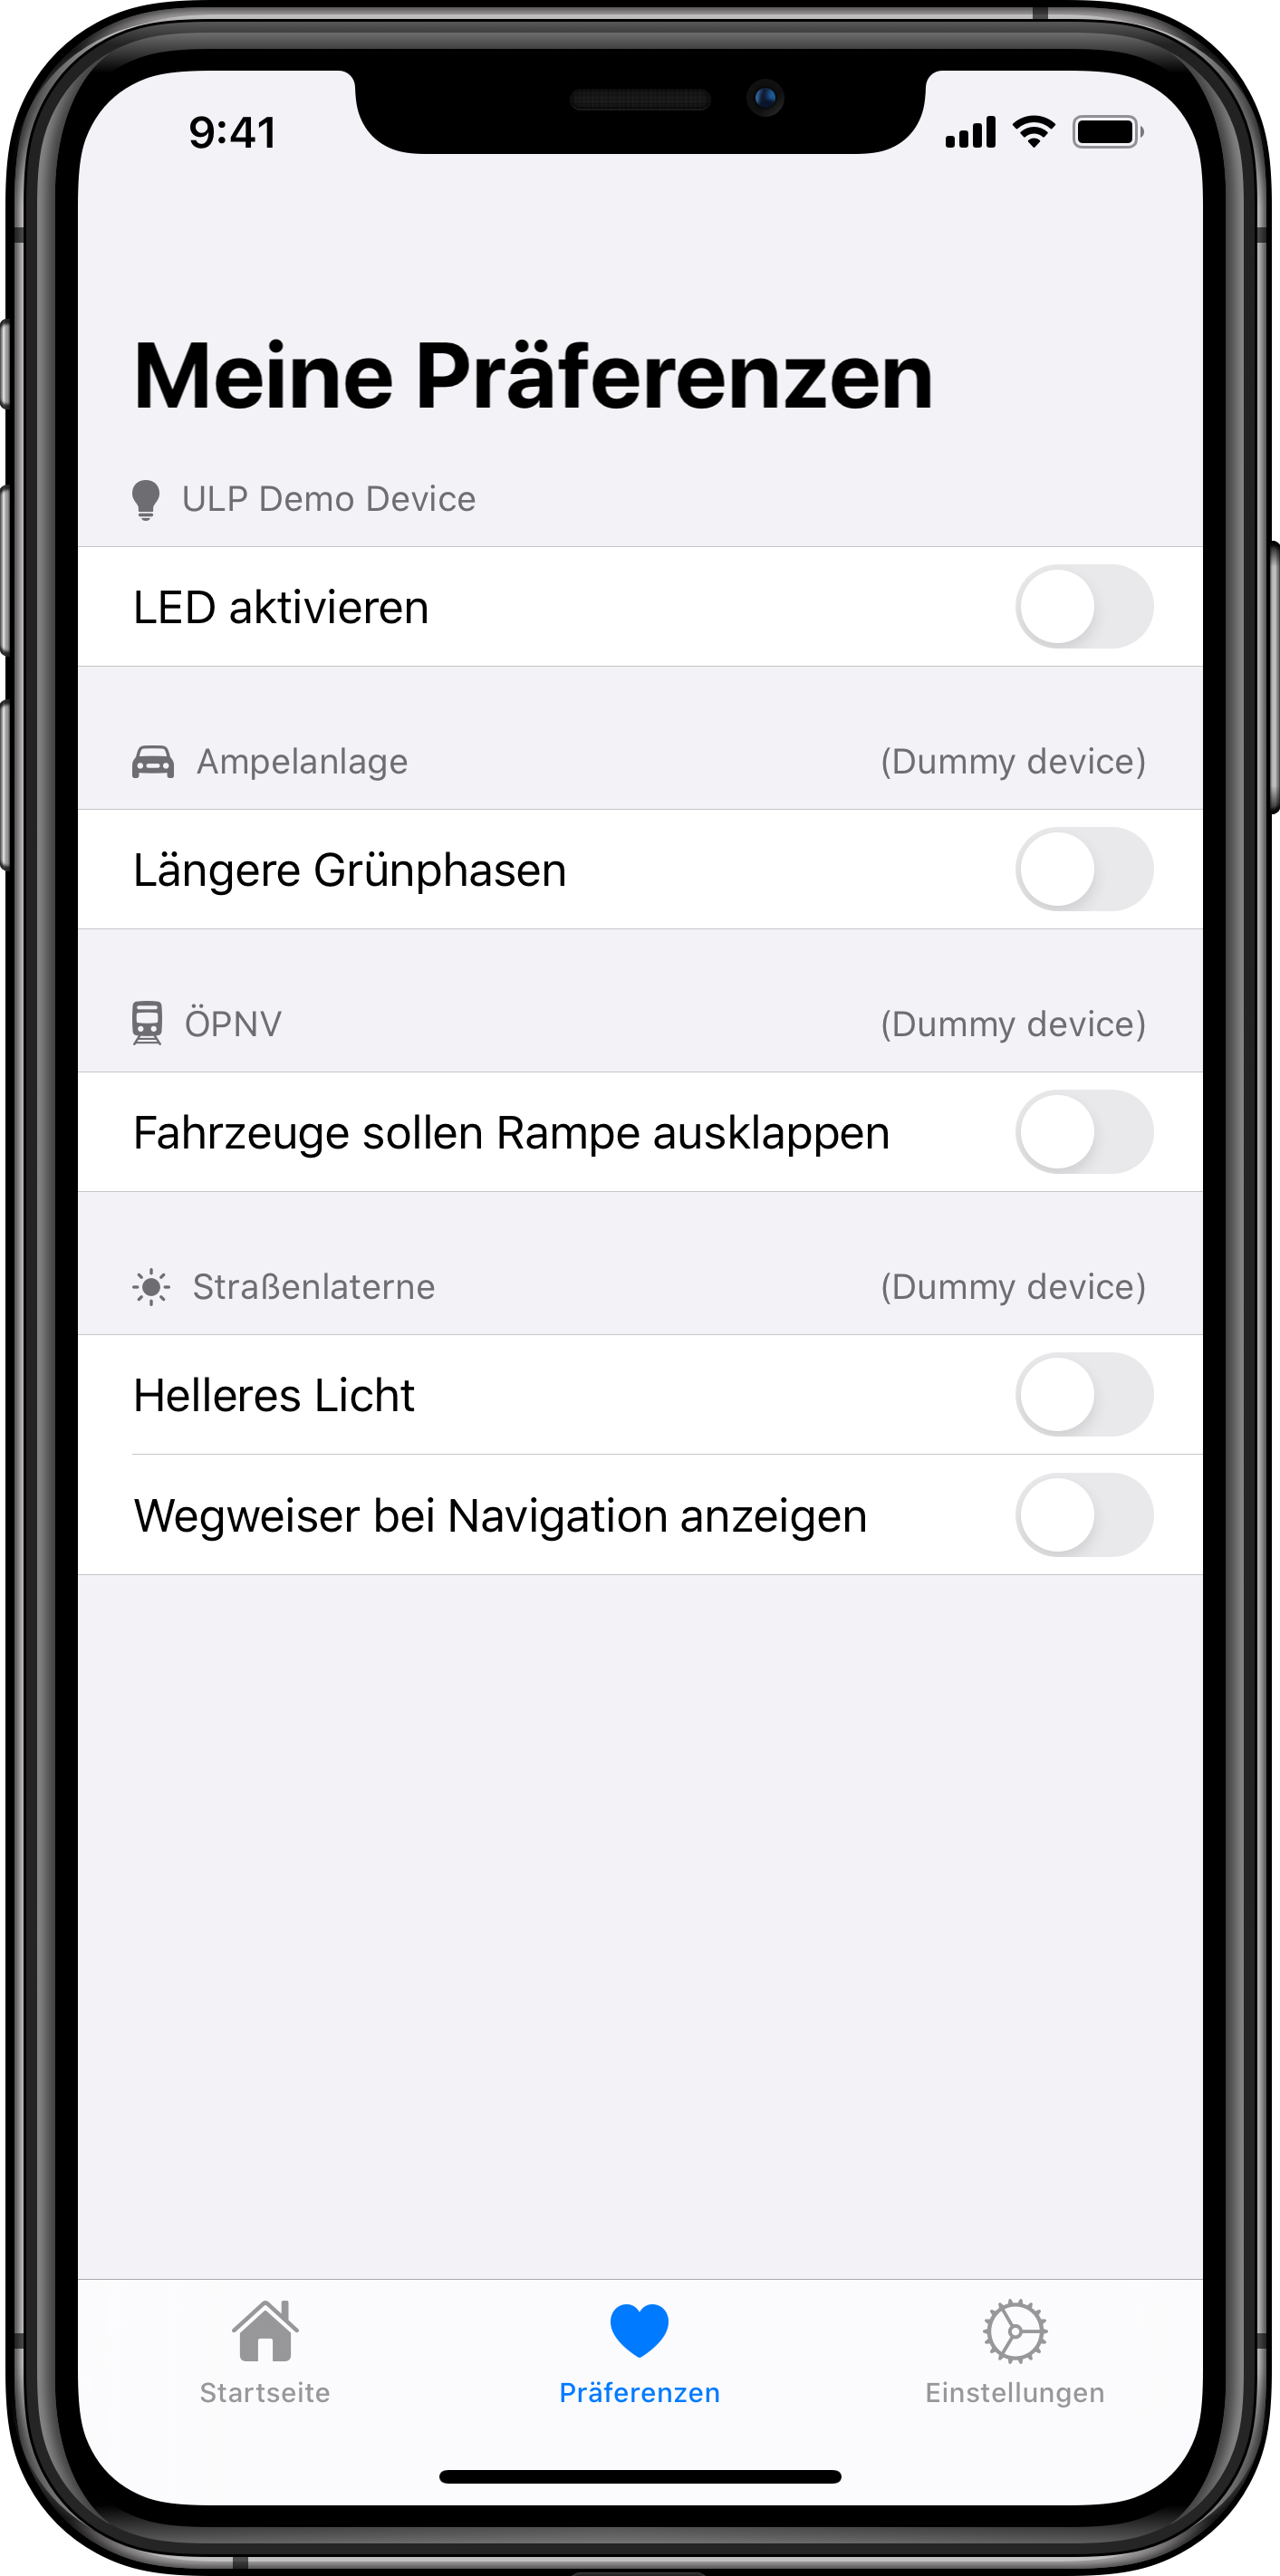
\includegraphics[width=.68\textwidth]{./images/prototype/ios/prefs.png}
		\caption{\label{fig:app:ios:prefs}Präferenzen festlegen.}
	\end{figure}
\end{minipage}\hfill
\begin{minipage}{.45\textwidth}
	\begin{figure}[H]
		\centering
		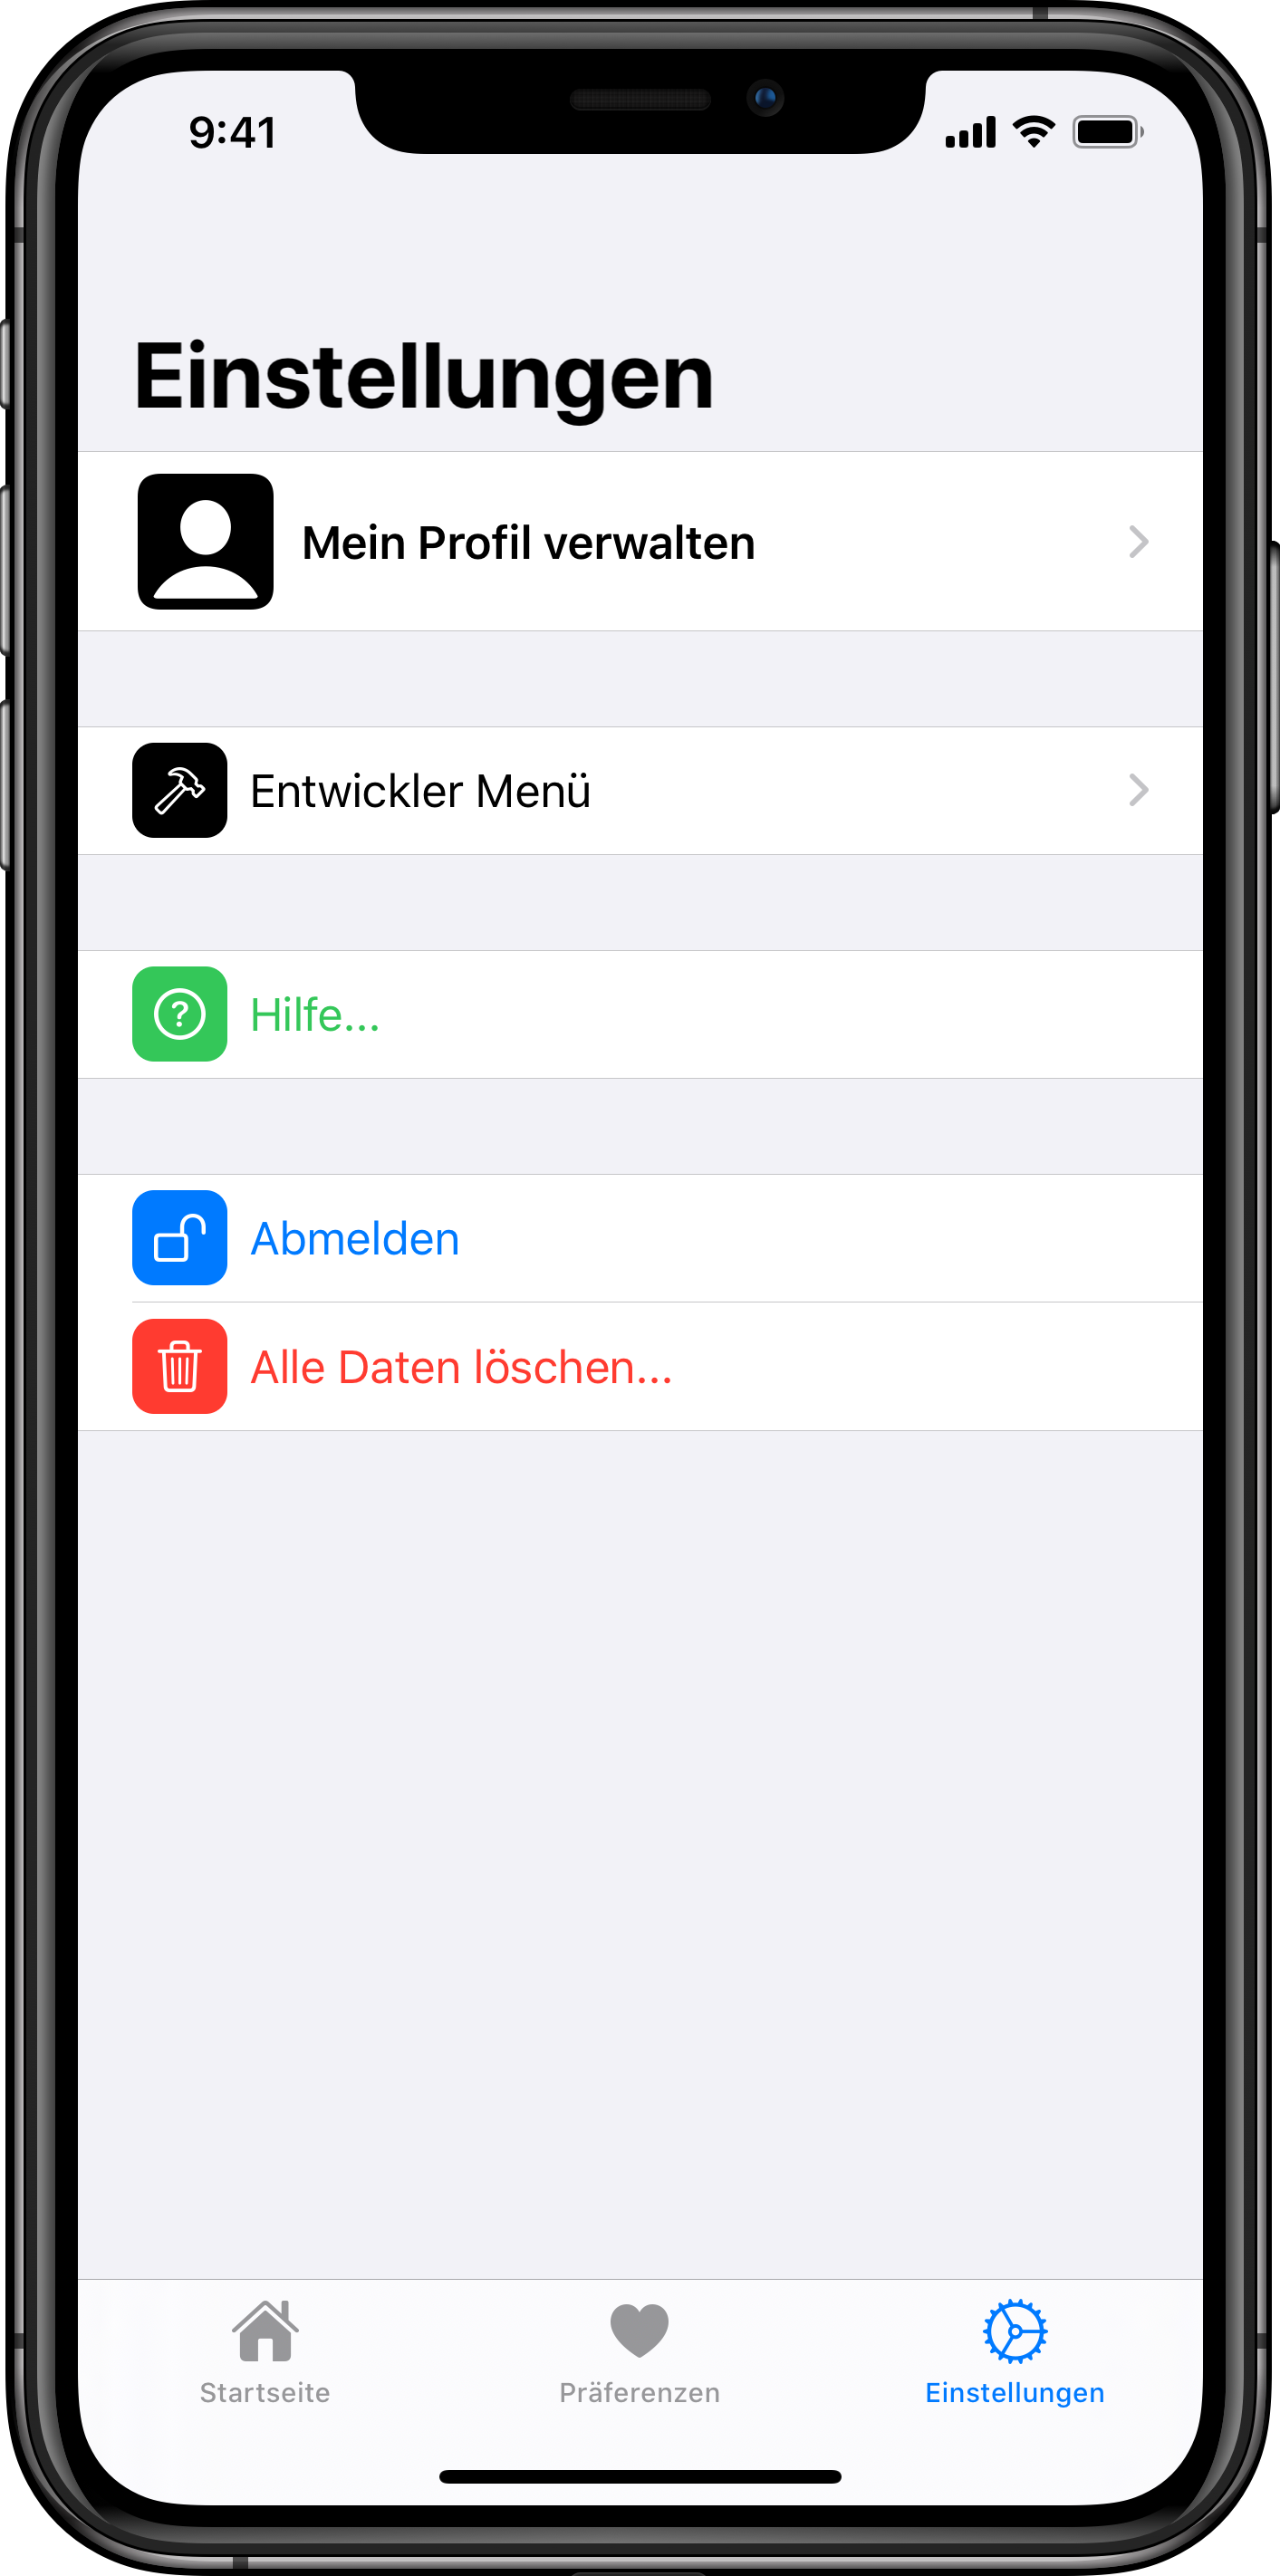
\includegraphics[width=.68\textwidth]{./images/prototype/ios/settings.png}
		\caption{\label{fig:app:ios:settings}Einstellungen der App.}
	\end{figure}
\end{minipage}

\begin{minipage}{.45\textwidth}
	\begin{figure}[H]
		\centering
		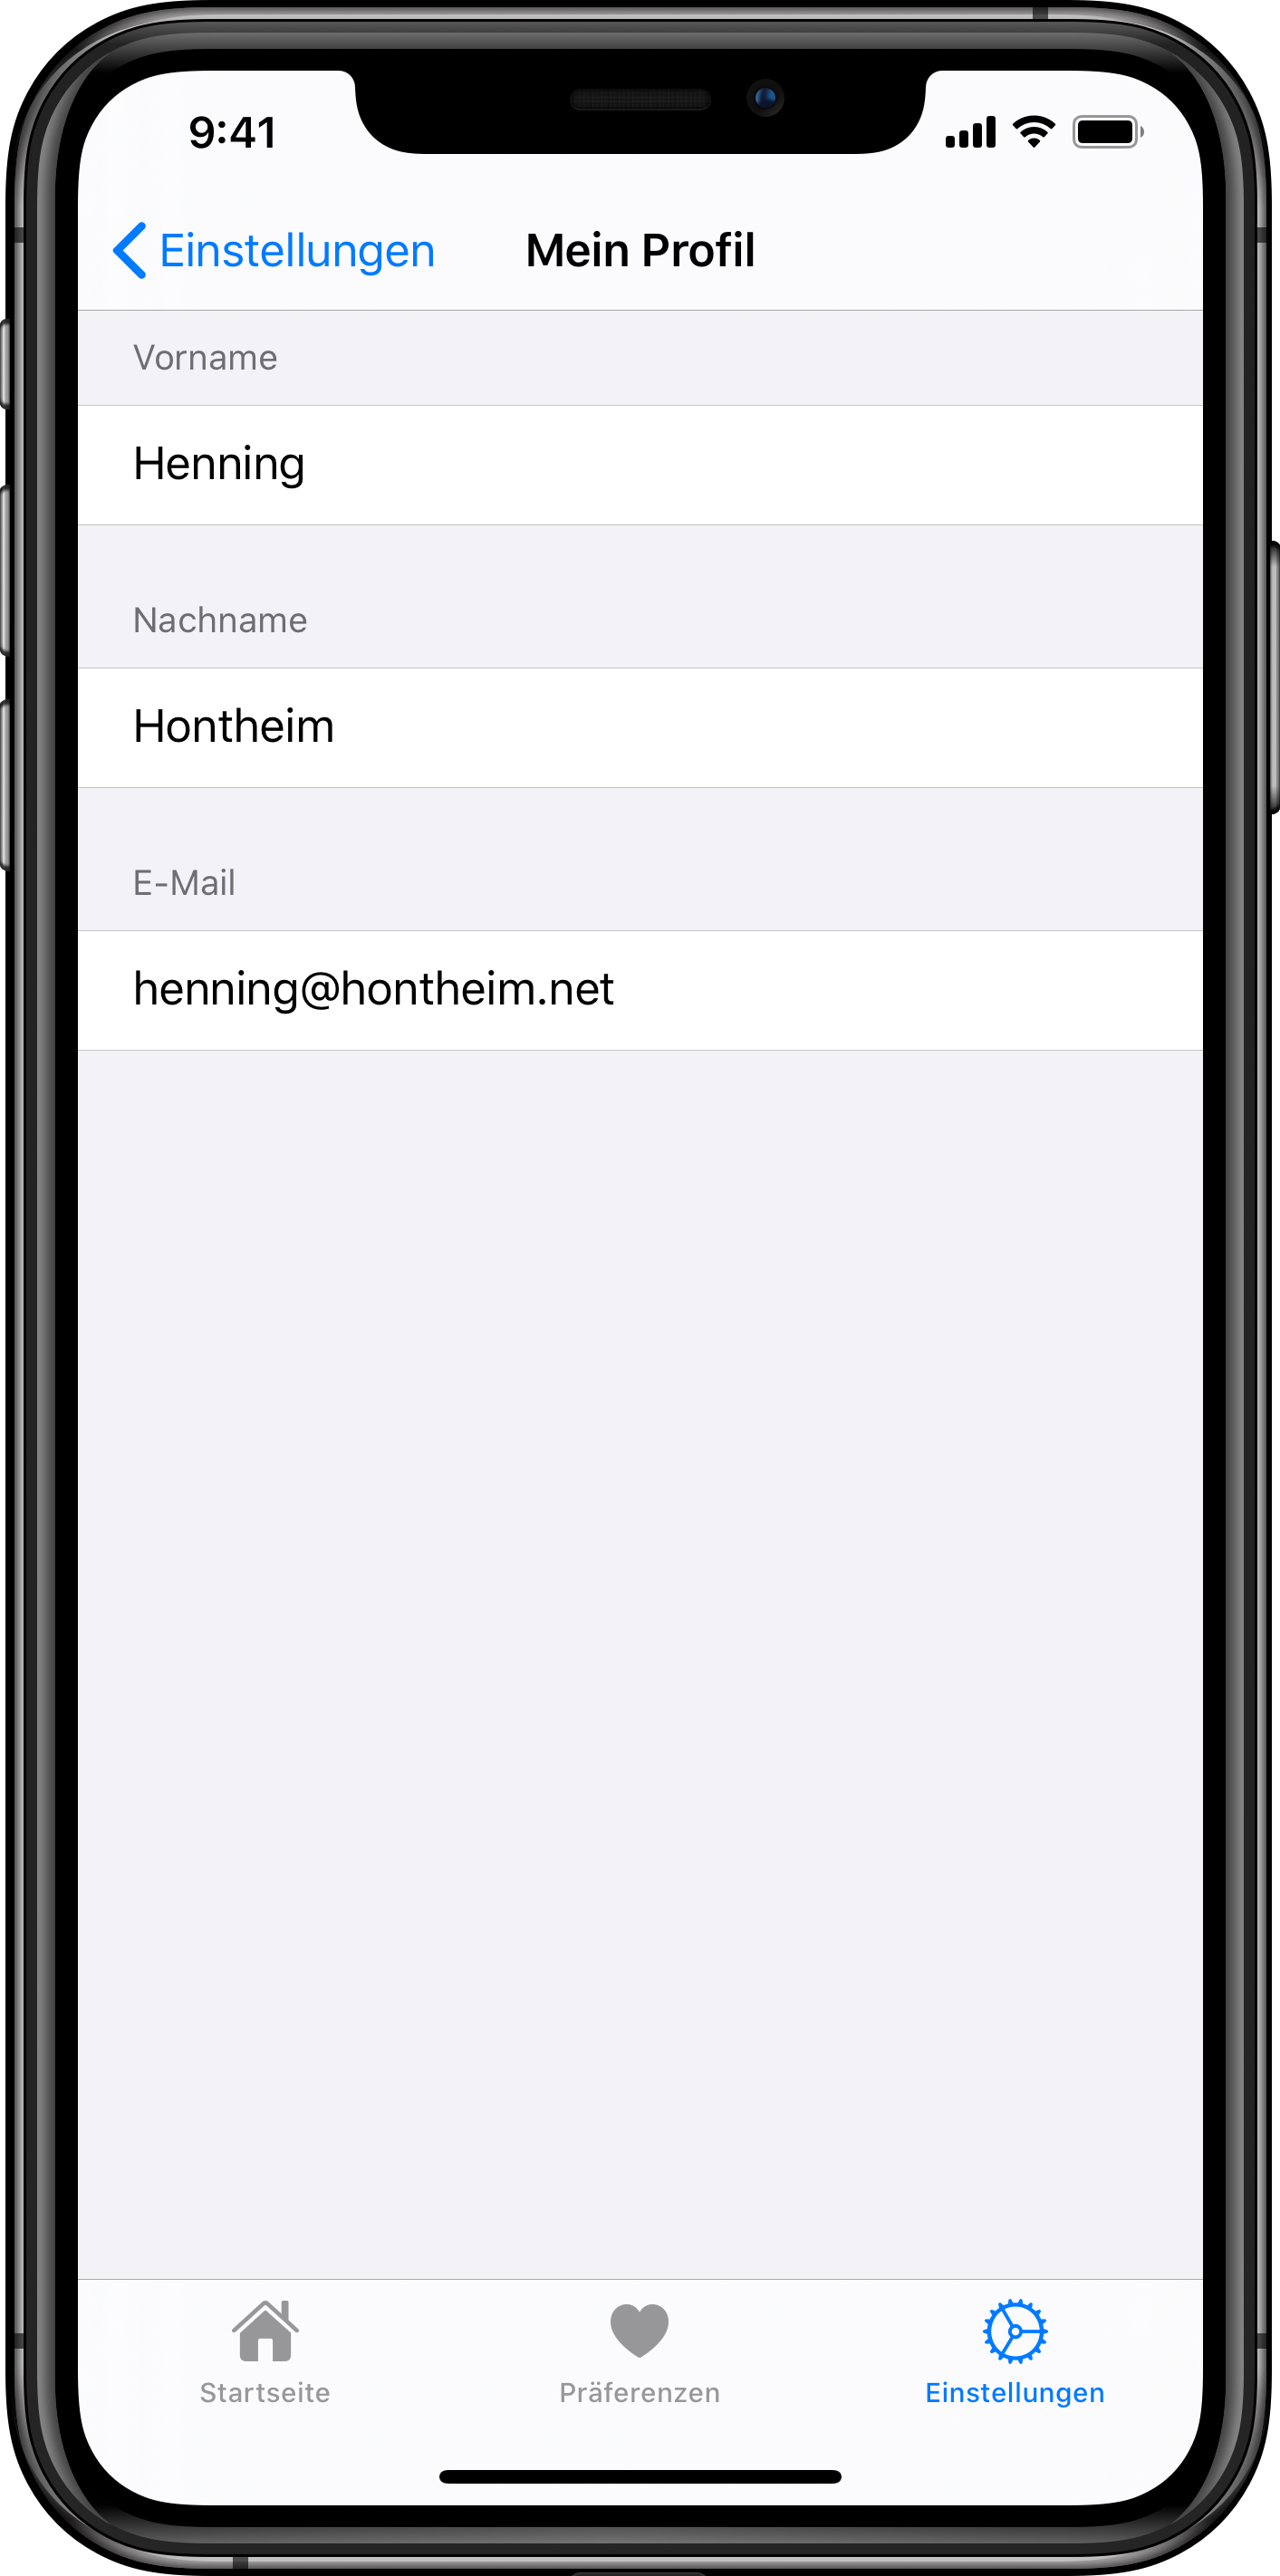
\includegraphics[width=.68\textwidth]{./images/prototype/ios/profile.png}
		\caption{\label{fig:app:ios:profile}Mein Profil verwalten.}
	\end{figure}
\end{minipage}\hfill
\begin{minipage}{.45\textwidth}
	\begin{figure}[H]
		\centering
		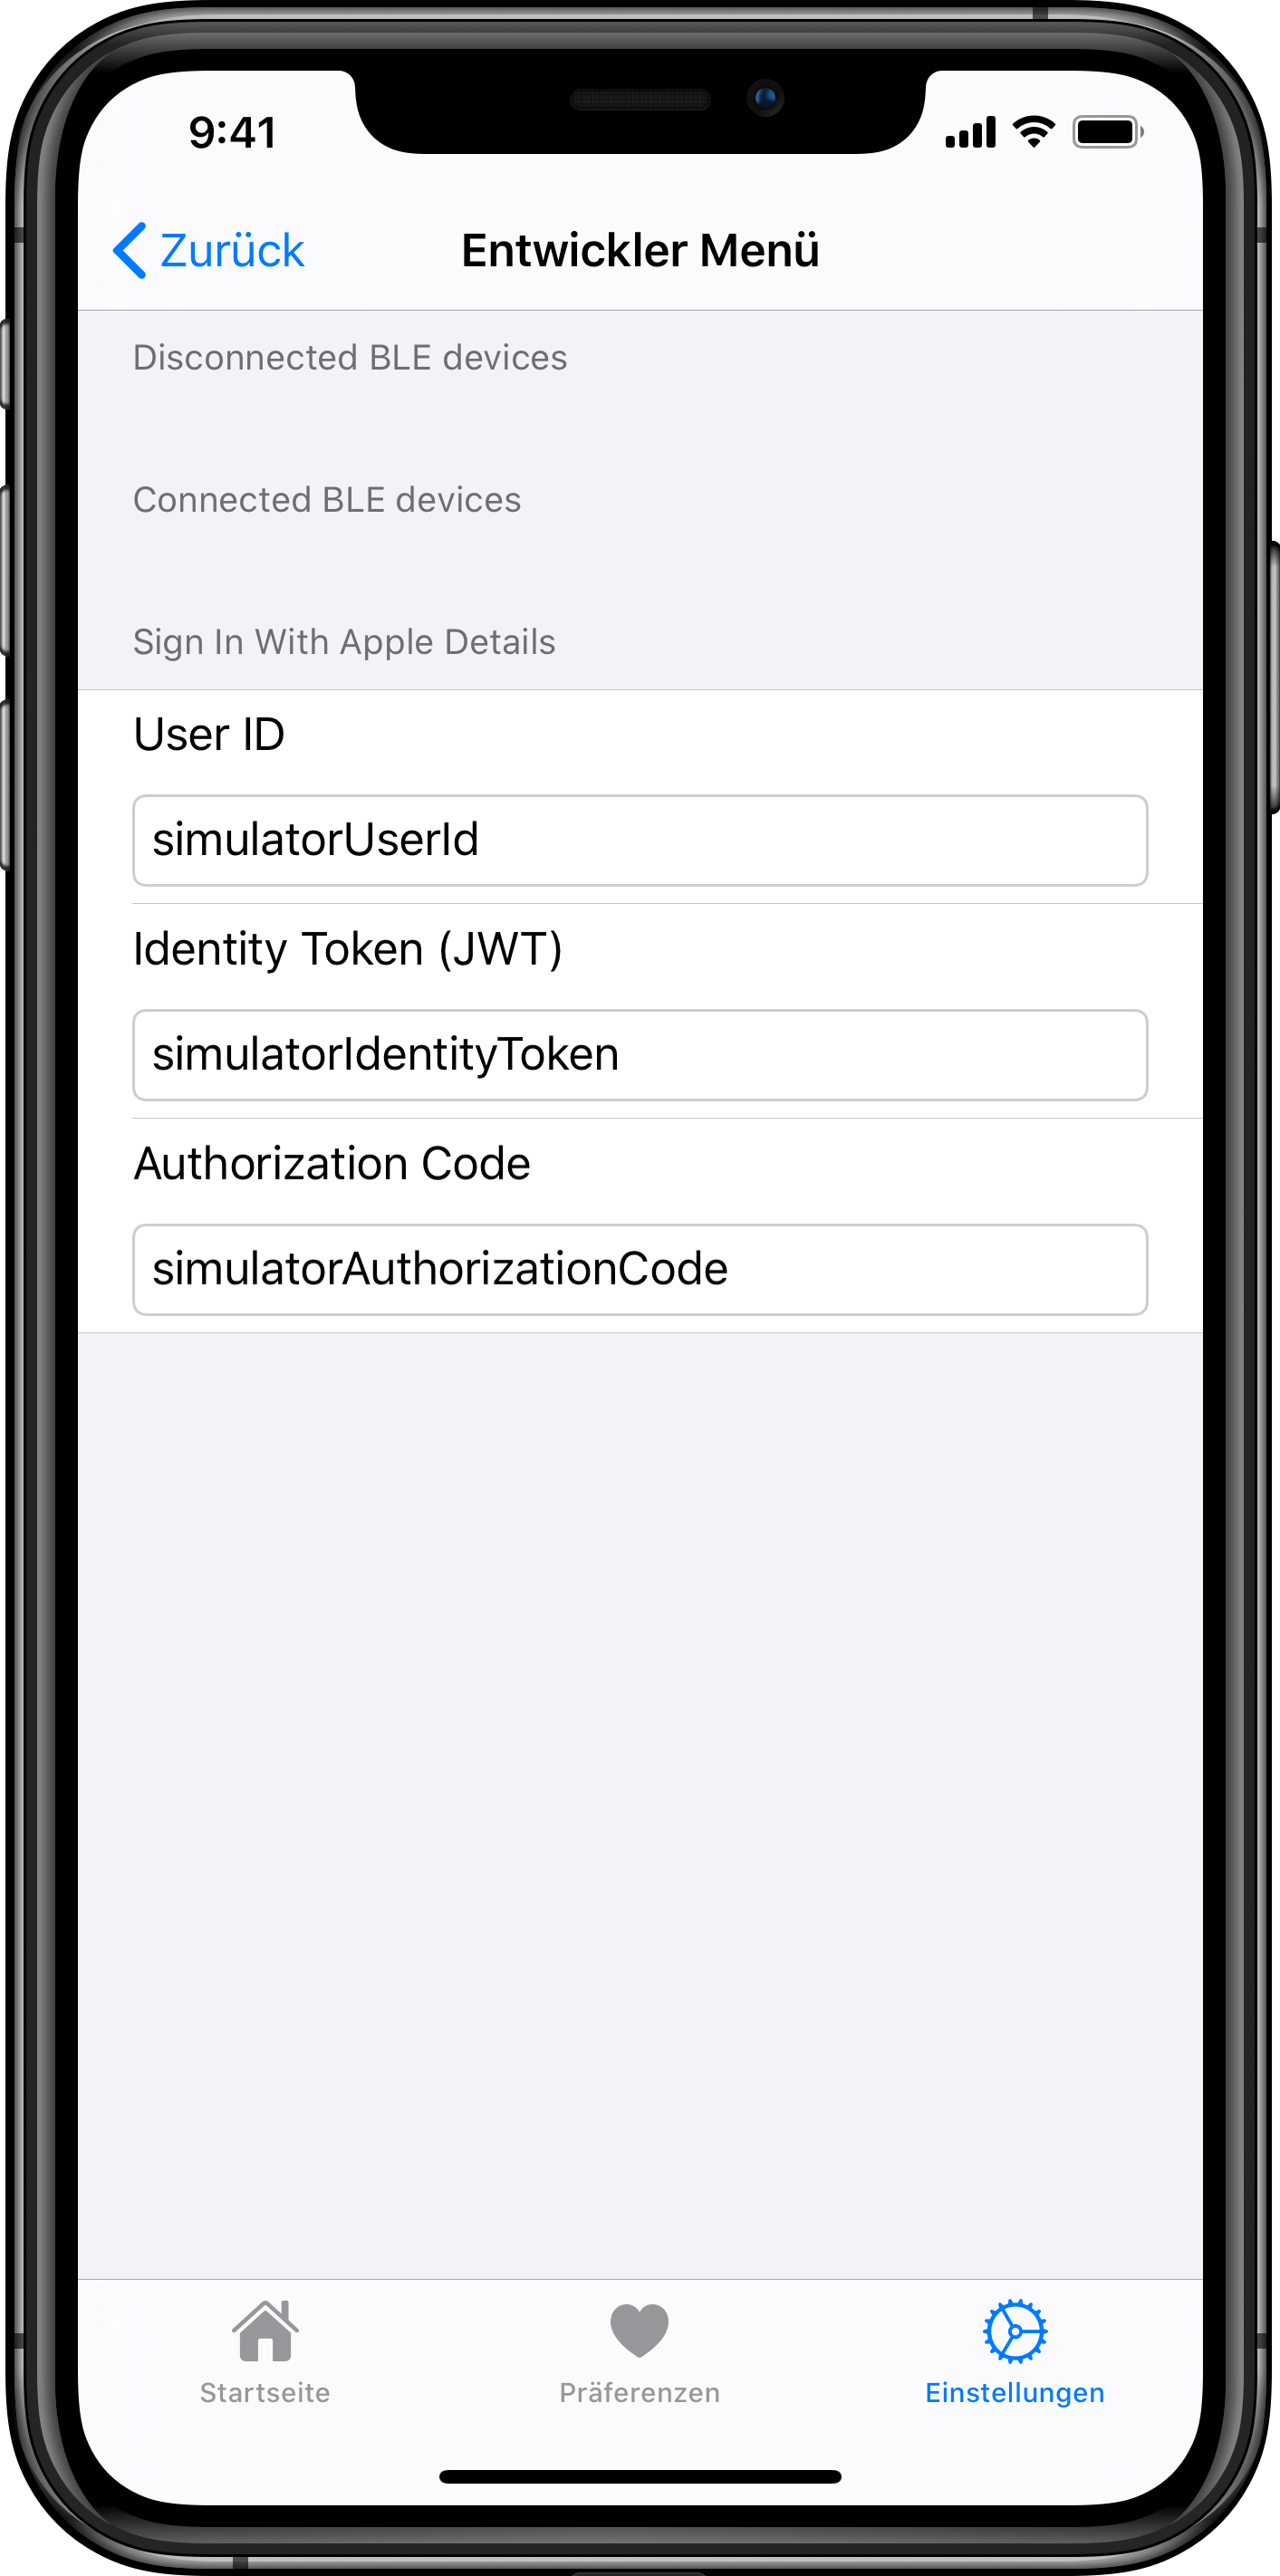
\includegraphics[width=.68\textwidth]{./images/prototype/ios/dev.png}
		\caption{\label{fig:app:ios:dev}Das Entwickler Menü.}
	\end{figure}
\end{minipage}

\begin{minipage}{.45\textwidth}
	\begin{figure}[H]
		\centering
		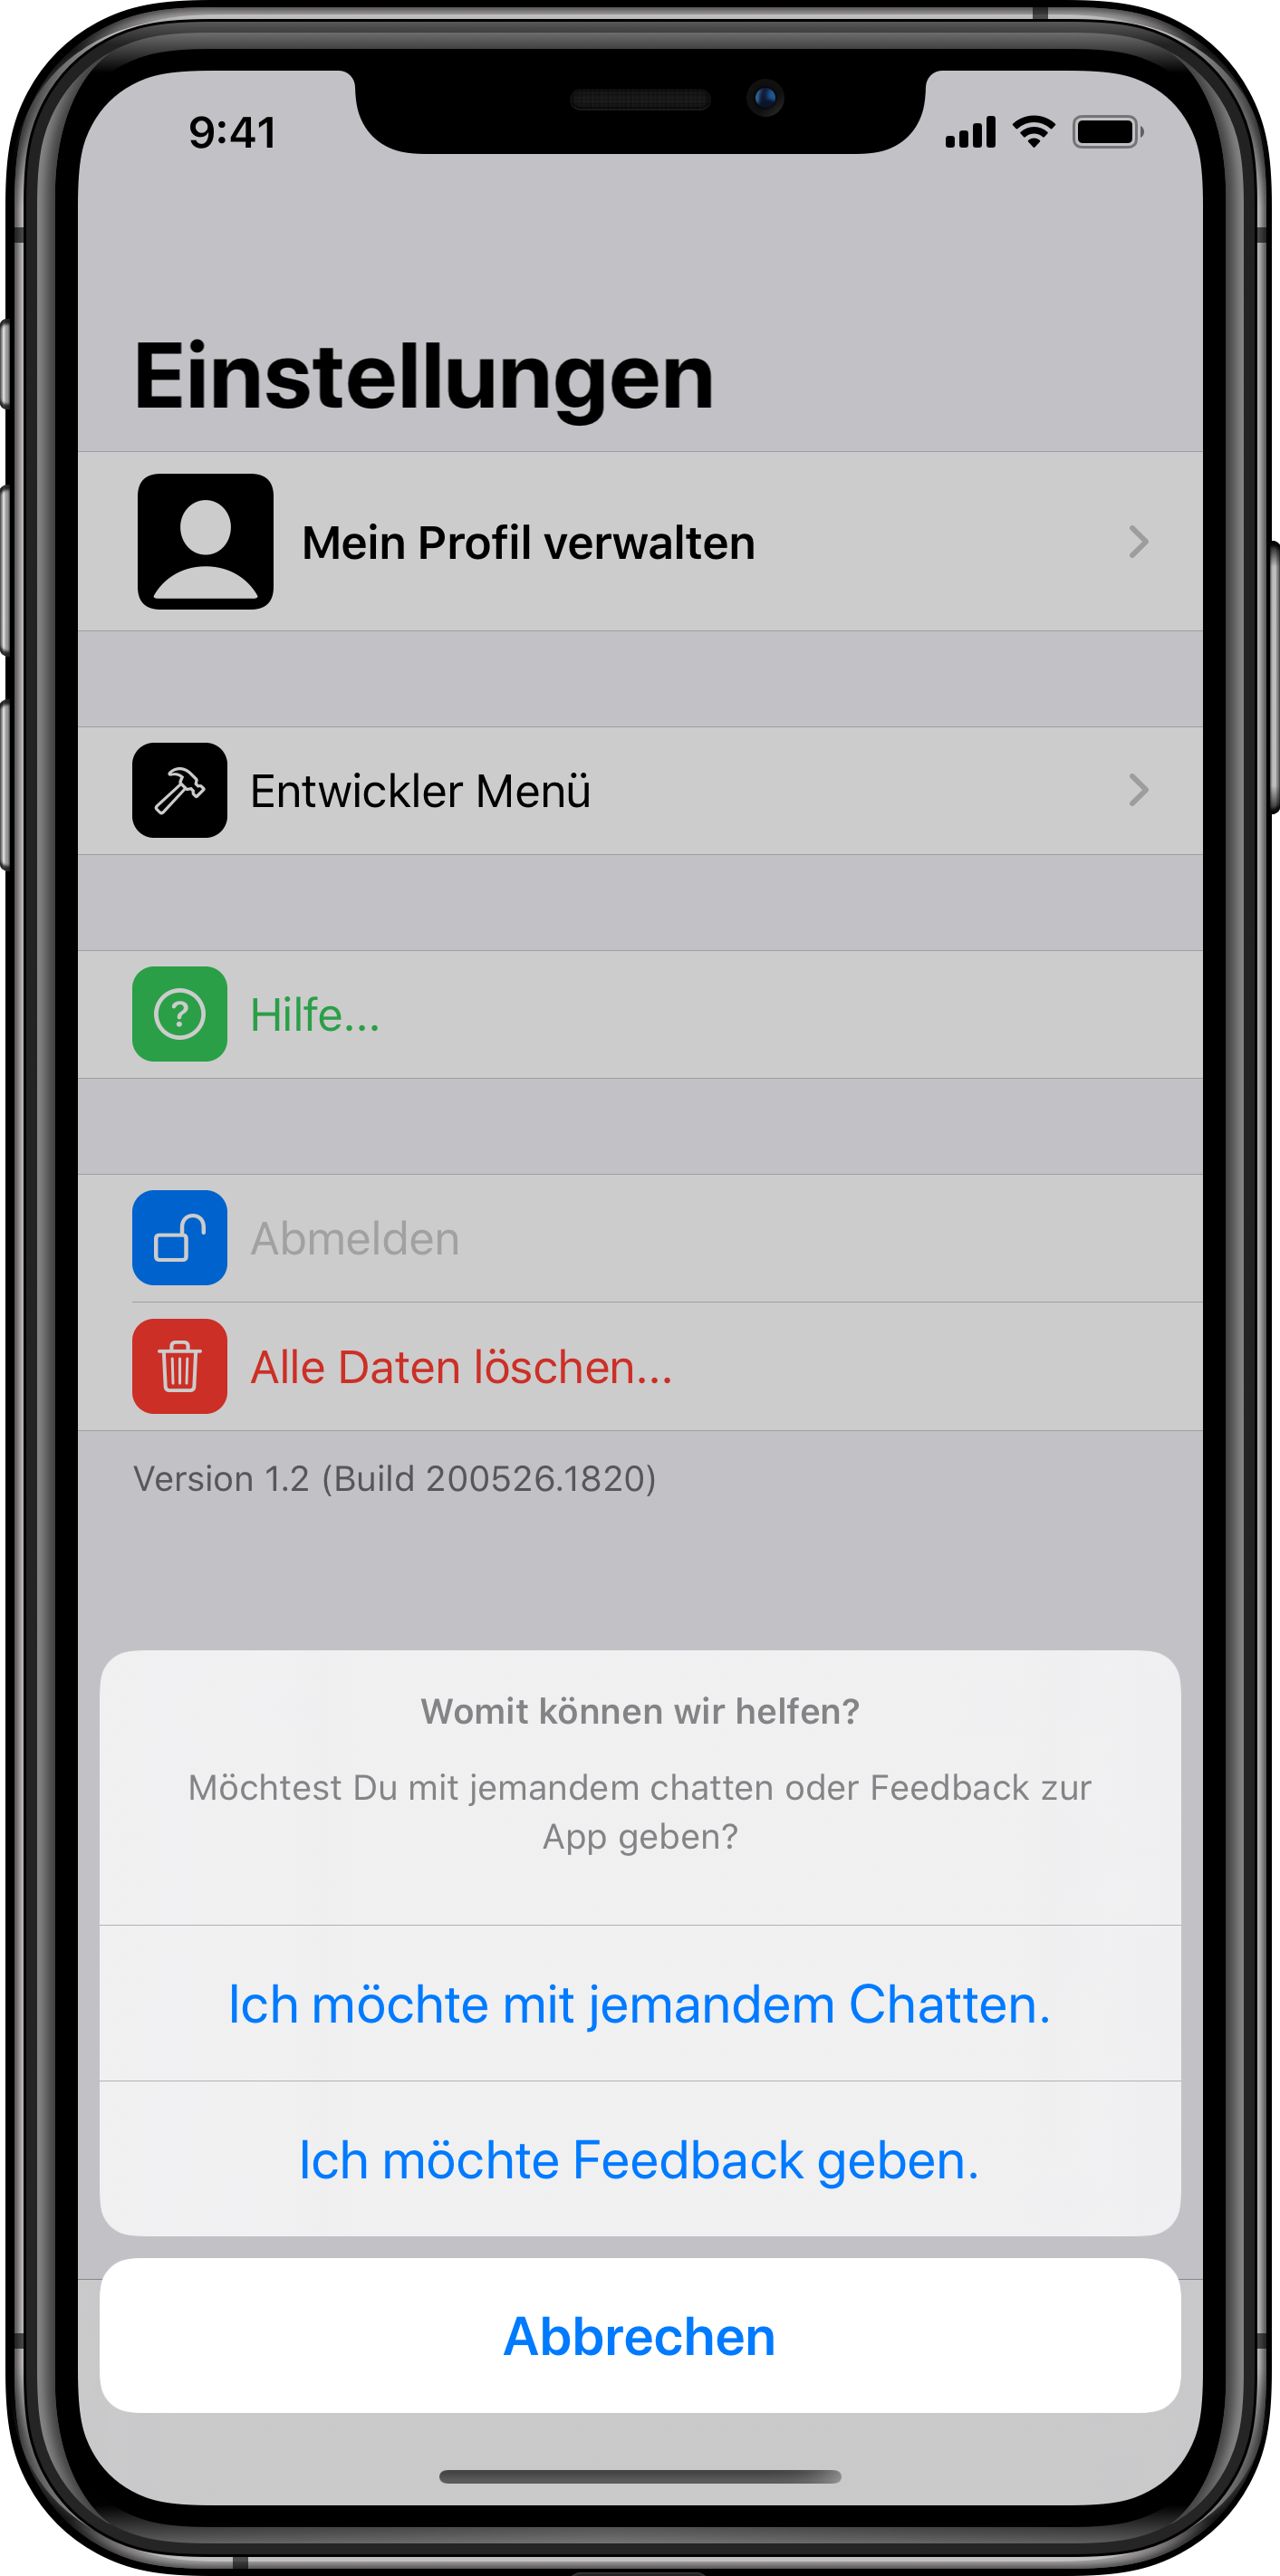
\includegraphics[width=.68\textwidth]{./images/prototype/ios/helpSheet.png}
		\caption{\label{fig:app:ios:helpSheet}Der Hilfe-Hinweis.}
	\end{figure}
\end{minipage}\hfill
\begin{minipage}{.45\textwidth}
	\begin{figure}[H]
		\centering
		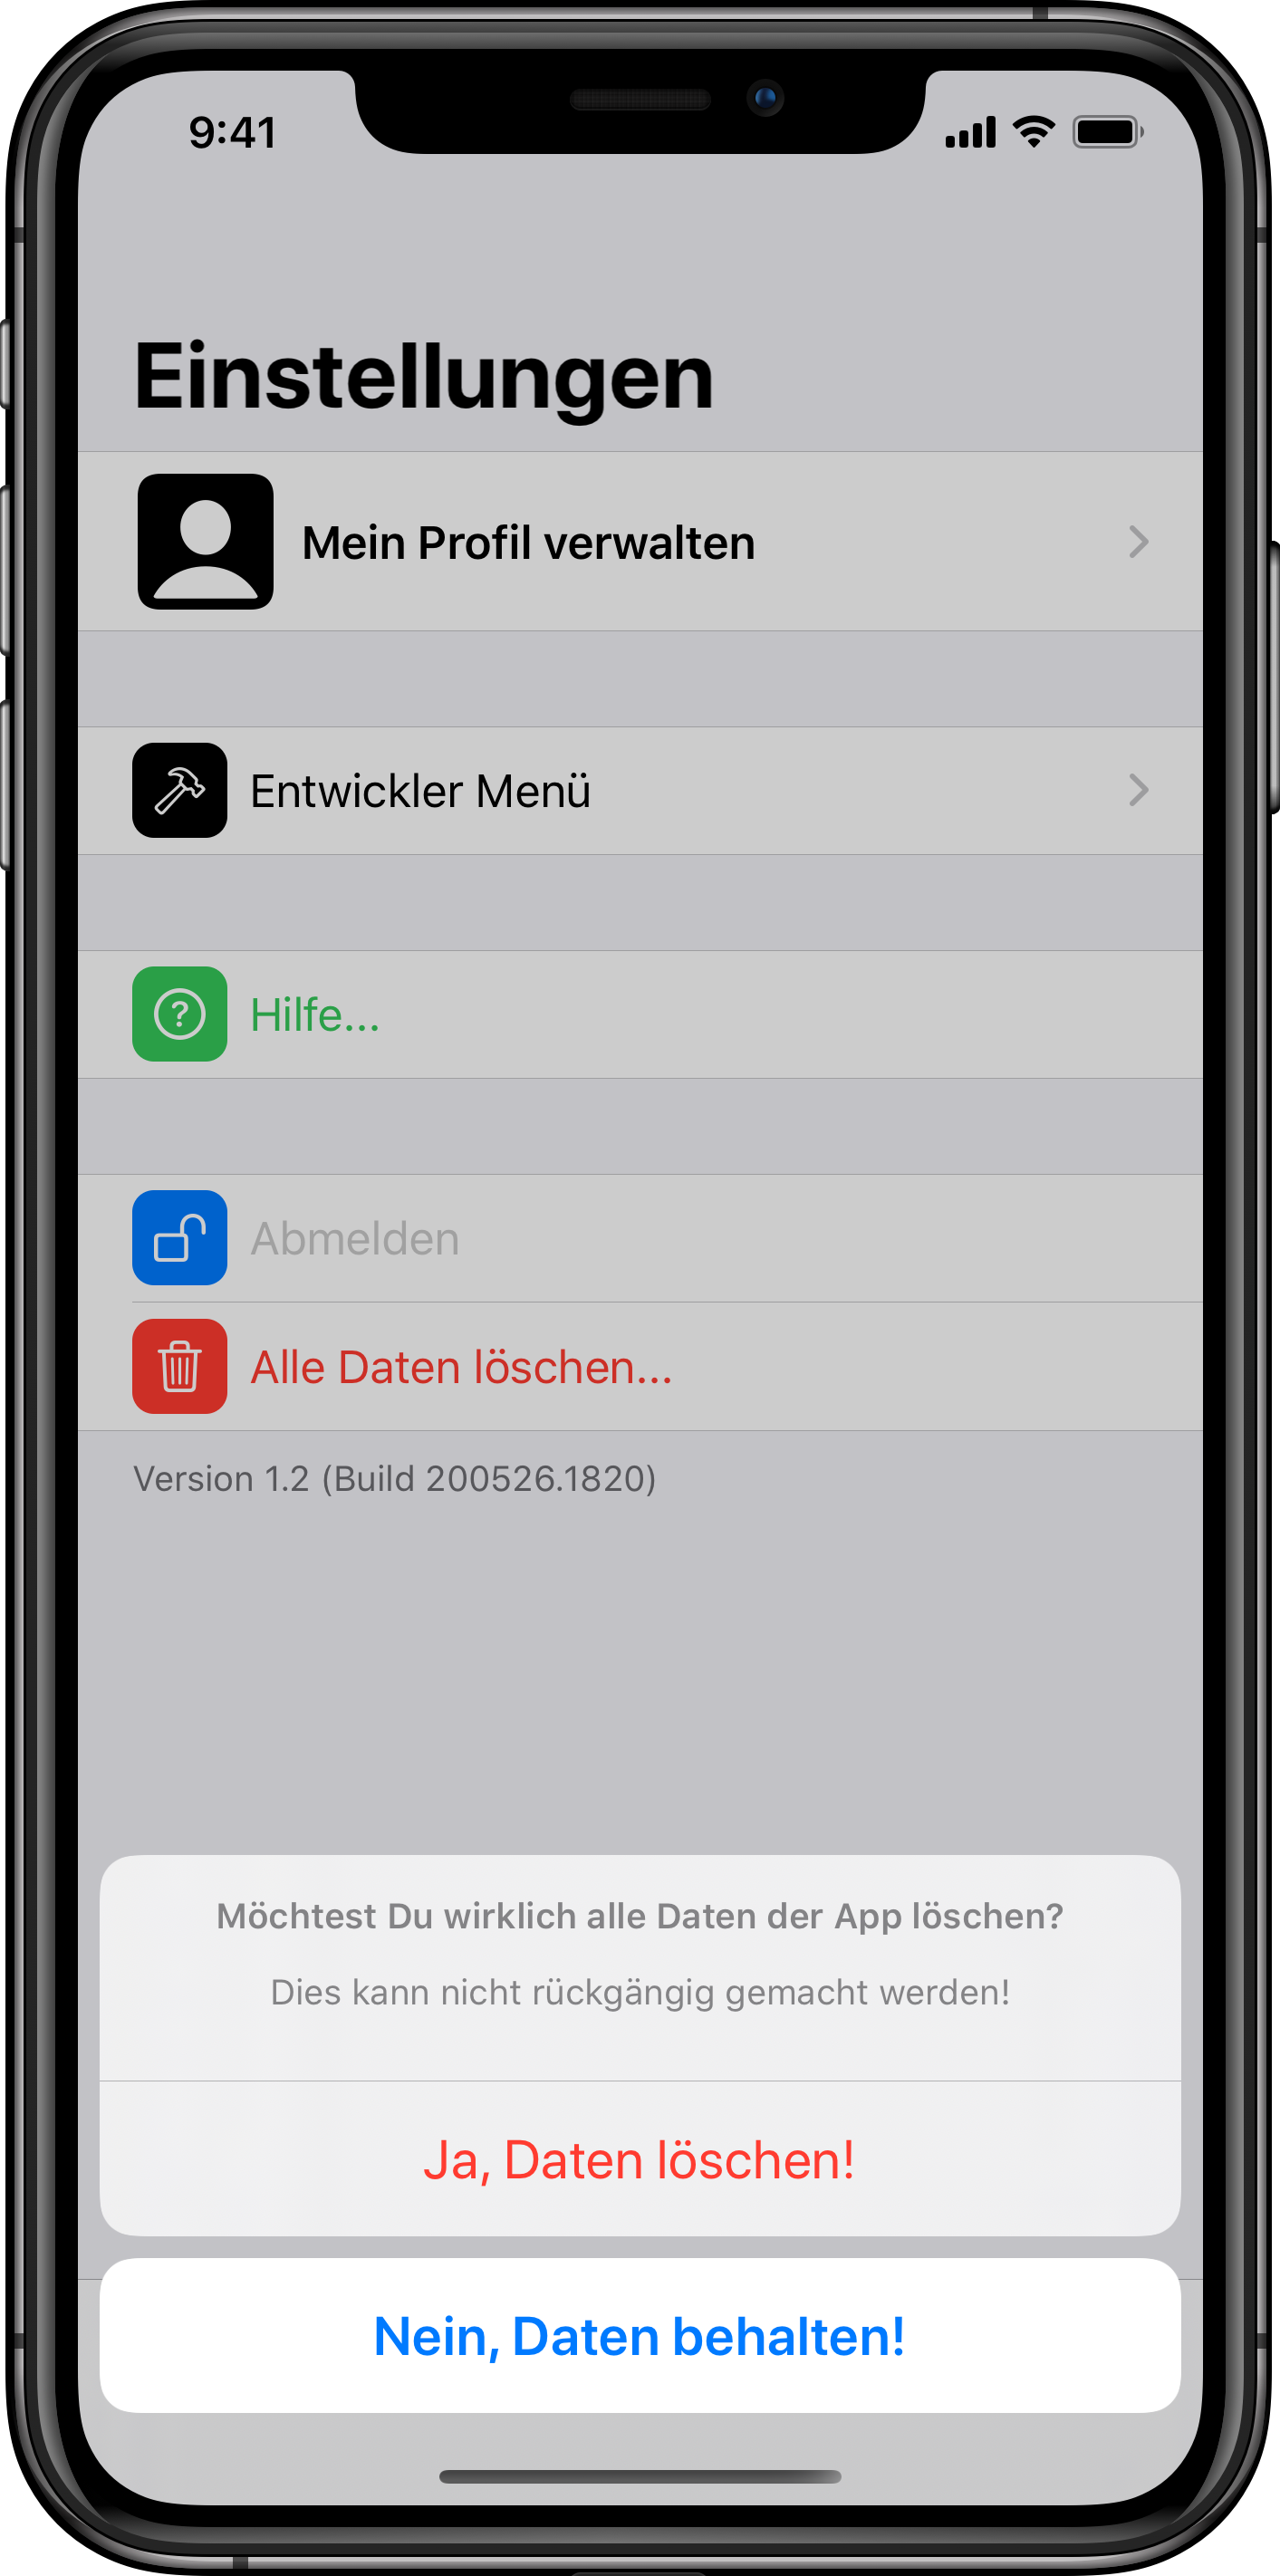
\includegraphics[width=.68\textwidth]{./images/prototype/ios/nukeSheet.png}
		\caption{\label{fig:app:ios:nukeSheet}Bestätigung der Datenlöschung.}
	\end{figure}
\end{minipage}

\begin{minipage}{.45\textwidth}
	\begin{figure}[H]
		\centering
		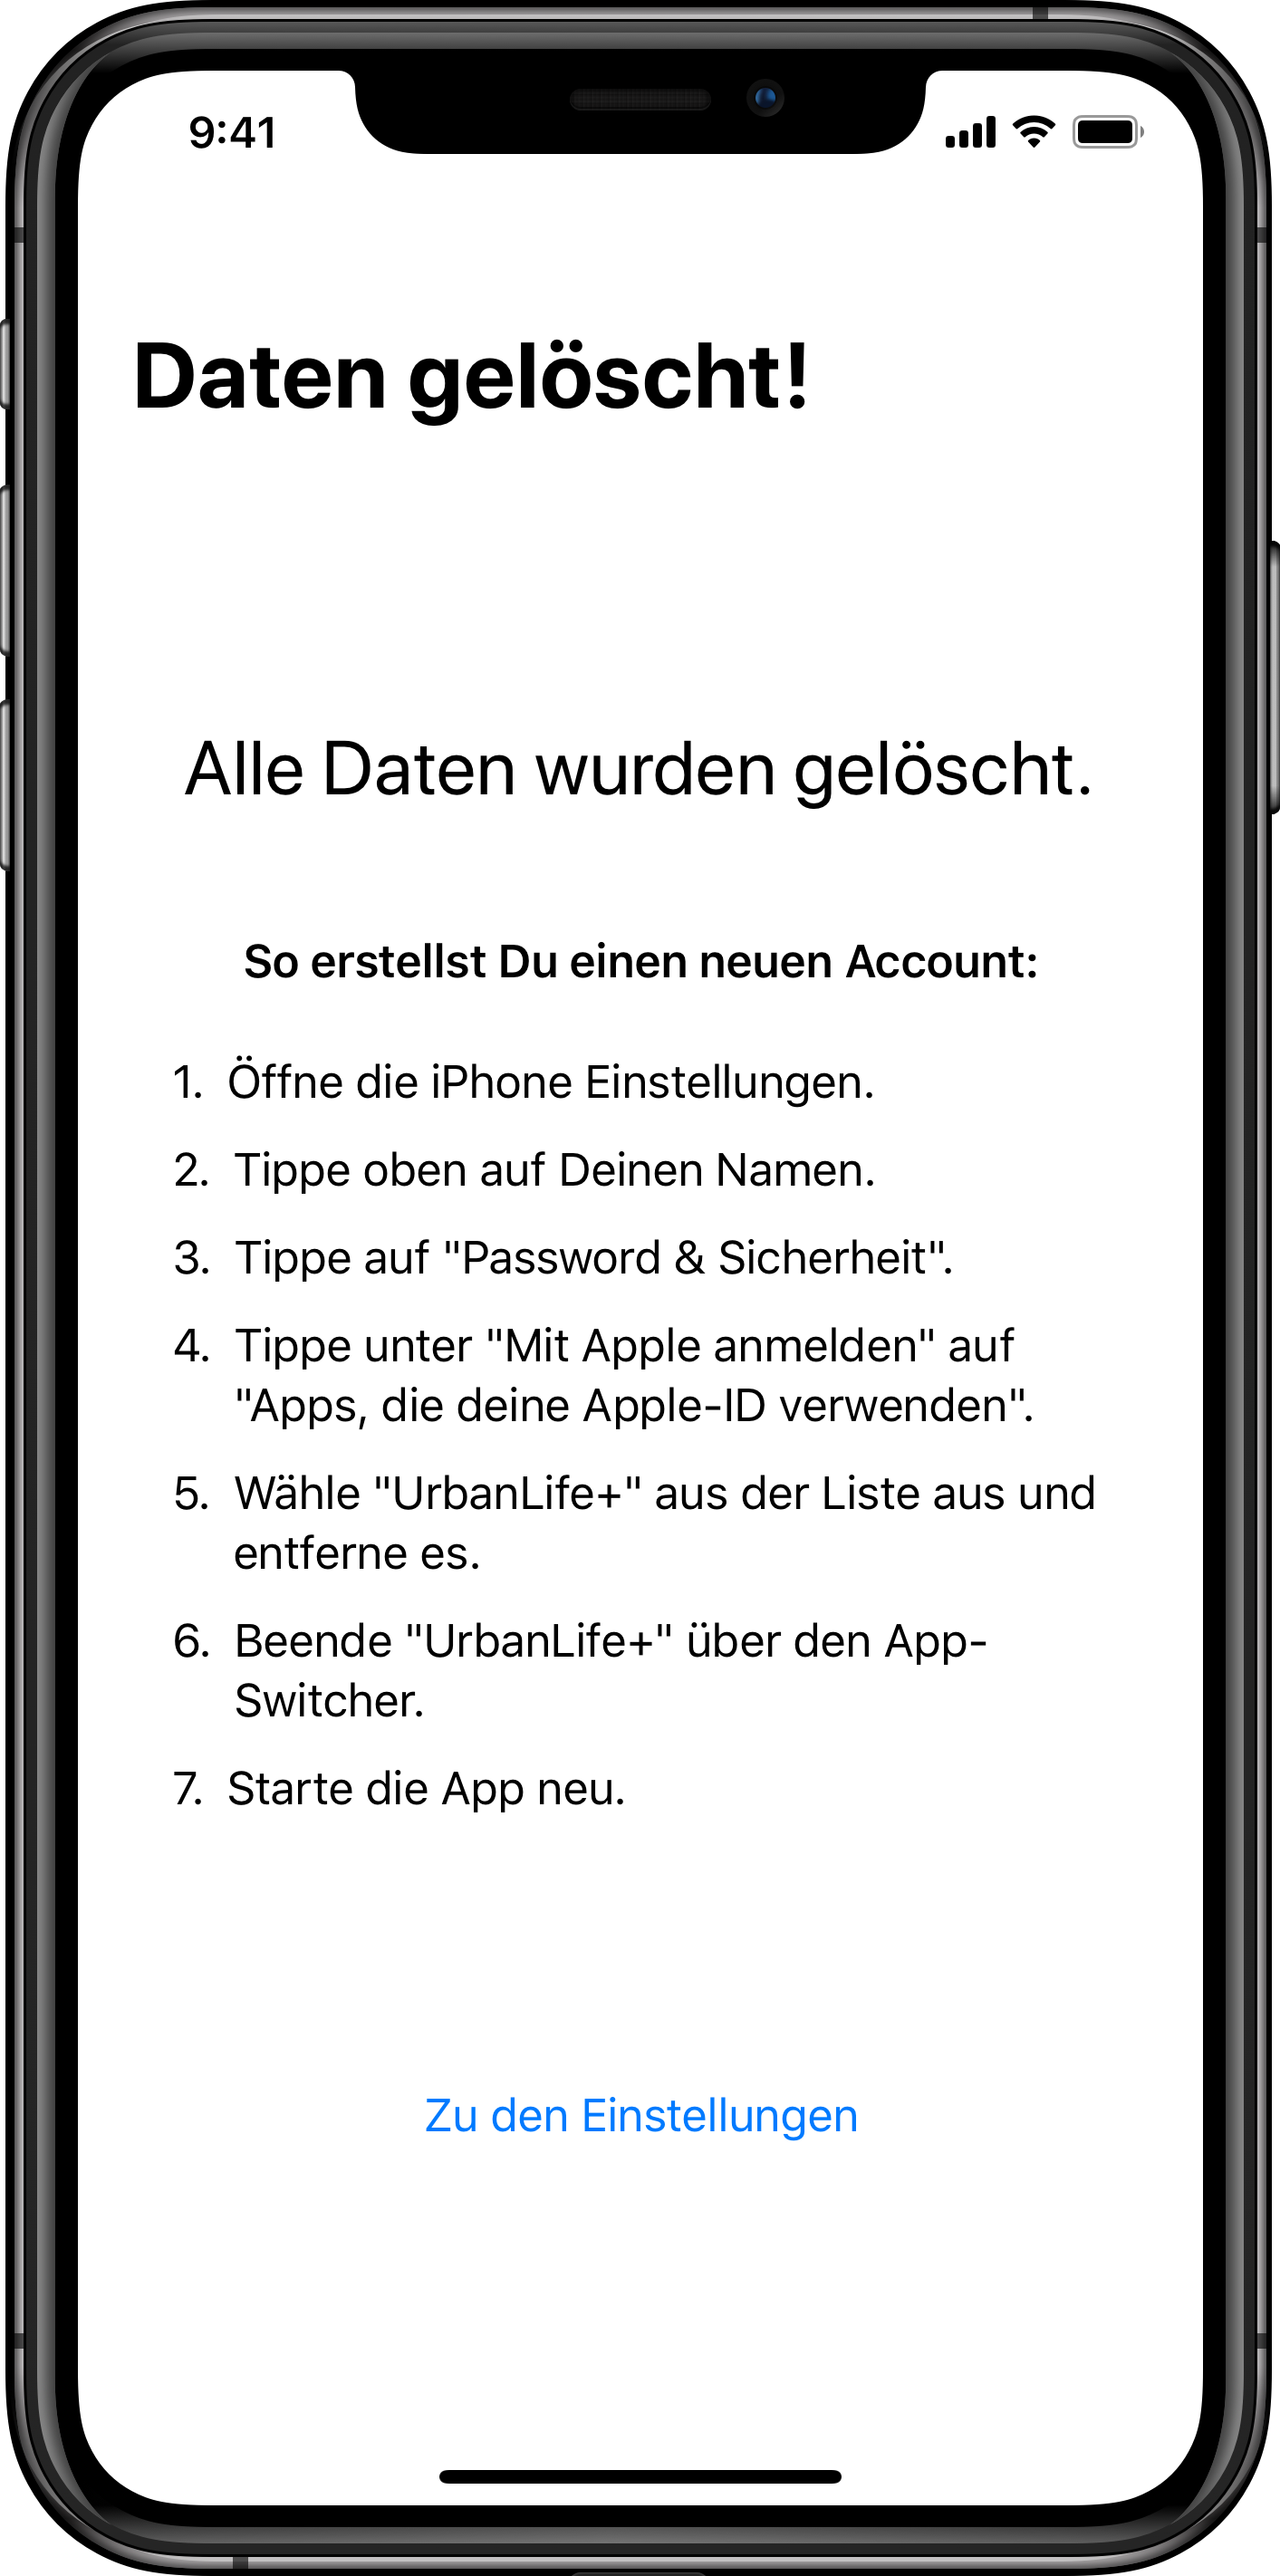
\includegraphics[width=.68\textwidth]{./images/prototype/ios/nuked.png}
		\caption{\label{fig:app:ios:nuked}Abschluss des Löschvorgangs.}
	\end{figure}
\end{minipage}

\subsection{watchOS App}

\begin{minipage}{.45\textwidth}
	\begin{figure}[H]
		\centering
		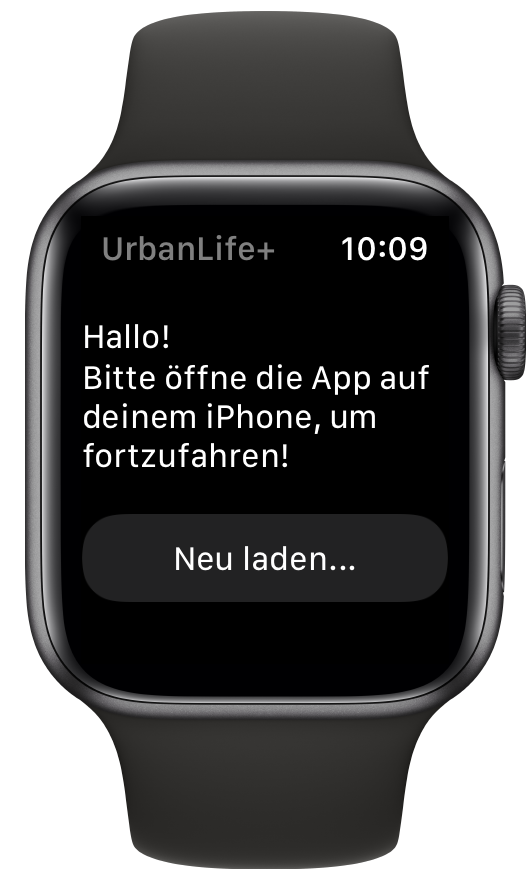
\includegraphics[width=.68\textwidth]{./images/prototype/watchos/loginNoAccount.png}
		\caption{\label{fig:app:watchos:loginNoAccount}Login-Screen. Benutzer hat noch keinen Account angelegt.}
	\end{figure}
\end{minipage}\hfill
\begin{minipage}{.45\textwidth}
	\begin{figure}[H]
		\centering
		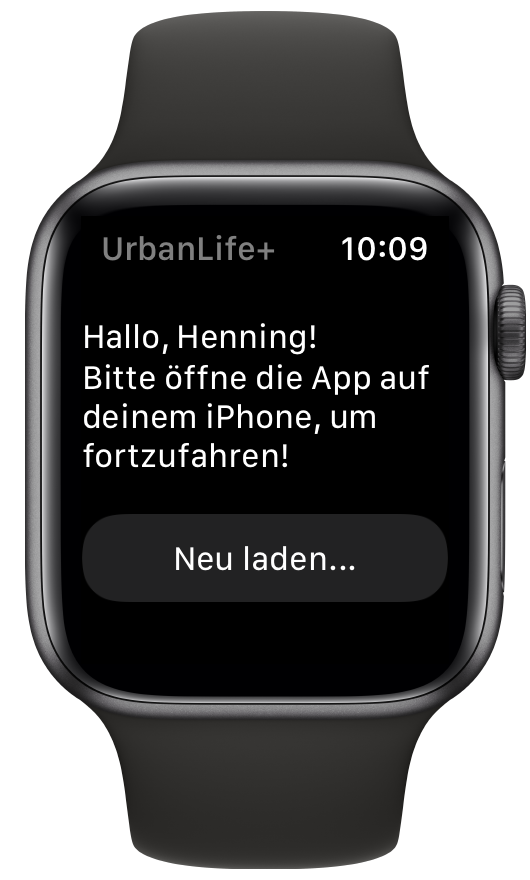
\includegraphics[width=.68\textwidth]{./images/prototype/watchos/loginWithAccount.png}
		\caption{\label{fig:app:watchos:loginWithAccount}Login-Screen. Benutzer hat bereits einen Account angelegt.}
	\end{figure}
\end{minipage}

\begin{minipage}{.45\textwidth}
	\begin{figure}[H]
		\centering
		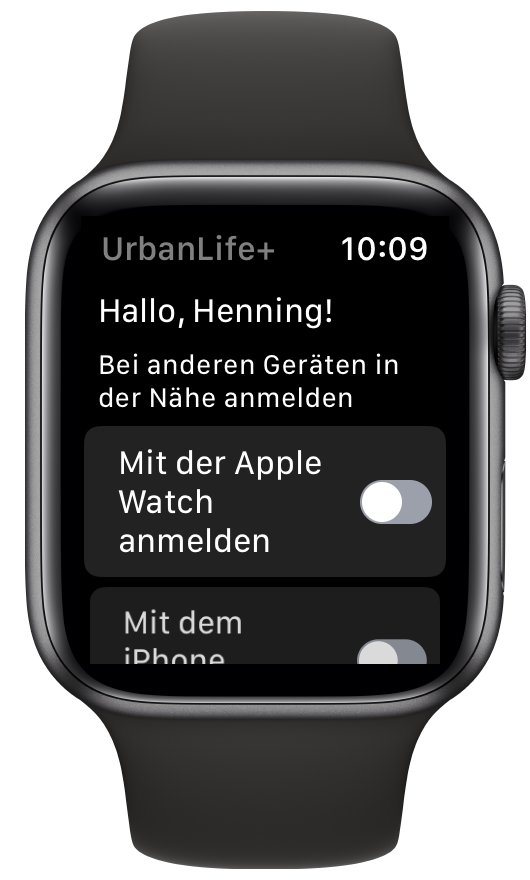
\includegraphics[width=.68\textwidth]{./images/prototype/watchos/home1.png}
		\caption{\label{fig:app:watchos:home1}Startseite. Teil 1.}
	\end{figure}
\end{minipage}\hfill
\begin{minipage}{.45\textwidth}
	\begin{figure}[H]
		\centering
		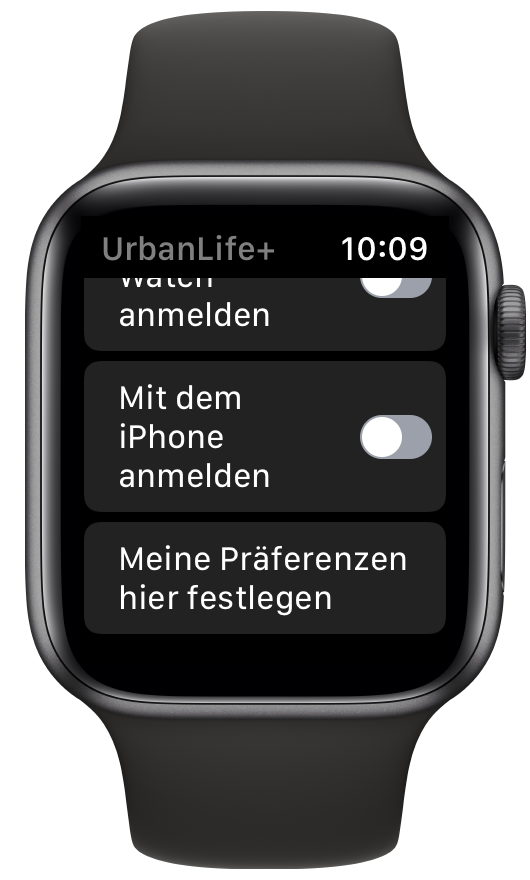
\includegraphics[width=.68\textwidth]{./images/prototype/watchos/home2.png}
		\caption{\label{fig:app:watchos:home2}Startseite. Teil 2.}
	\end{figure}
\end{minipage}

\begin{minipage}{.45\textwidth}
	\begin{figure}[H]
		\centering
		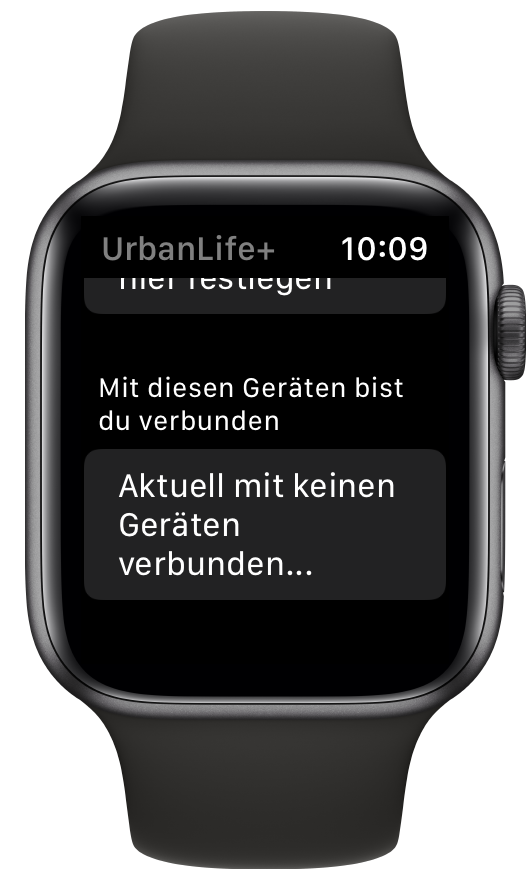
\includegraphics[width=.68\textwidth]{./images/prototype/watchos/homeNotConnected.png}
		\caption{\label{fig:app:watchos:homeNotConnected}Startseite. Uhr ist nicht mit Gerät verbunden.}
	\end{figure}
\end{minipage}\hfill
\begin{minipage}{.45\textwidth}
	\begin{figure}[H]
		\centering
		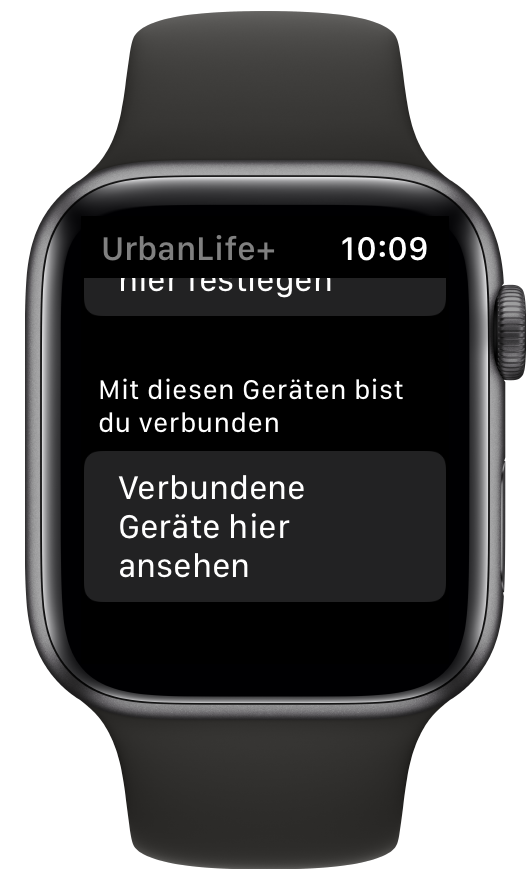
\includegraphics[width=.68\textwidth]{./images/prototype/watchos/homeIsConnected.png}
		\caption{\label{fig:app:watchos:homeIsConnected}Startseite. Uhr ist mit einem Gerät verbunden.}
	\end{figure}
\end{minipage}

\begin{minipage}{.45\textwidth}
	\begin{figure}[H]
		\centering
		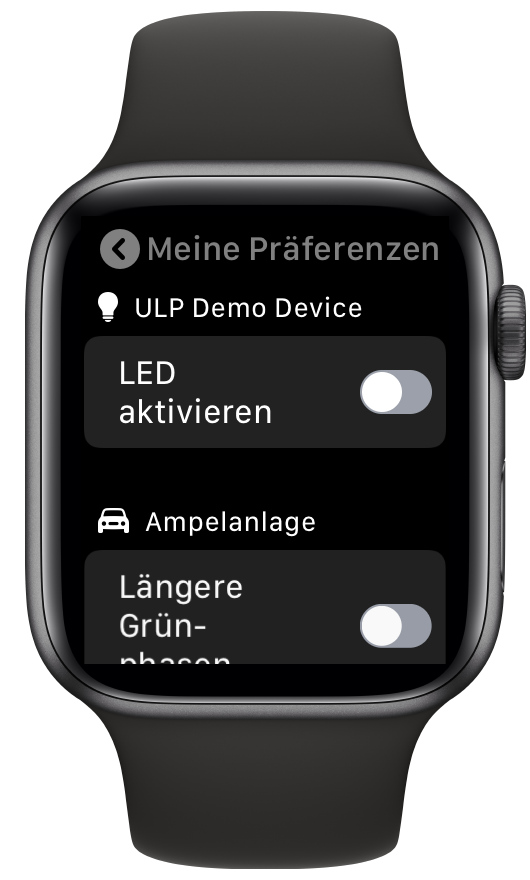
\includegraphics[width=.68\textwidth]{./images/prototype/watchos/prefs.png}
		\caption{\label{fig:app:watchos:prefs}Präferenzen festlegen.}
	\end{figure}
\end{minipage}\hfill
\begin{minipage}{.45\textwidth}
	\begin{figure}[H]
		\centering
		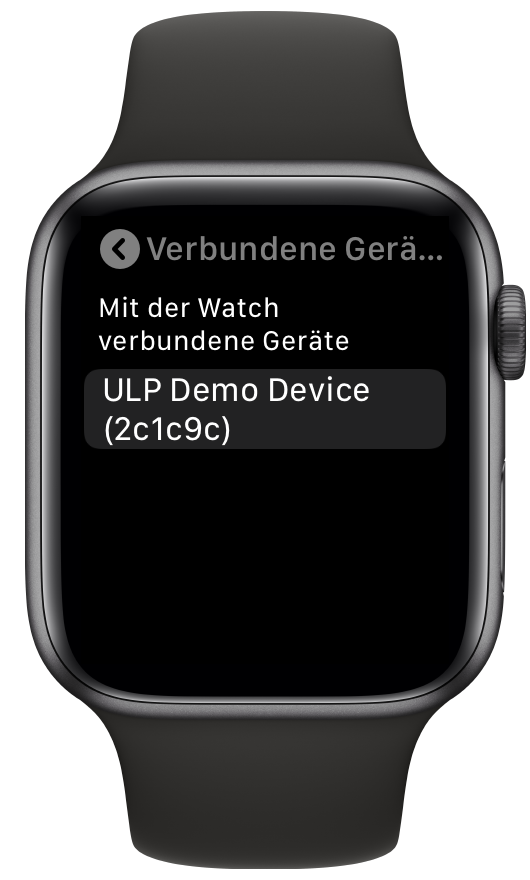
\includegraphics[width=.68\textwidth]{./images/prototype/watchos/connectedTo.png}
		\caption{\label{fig:app:watchos:connectedTo}Verbundene Geräte.}
	\end{figure}
\end{minipage}
